\pdfoptionpdfminorversion=5
\documentclass[10pt]{book}

\usepackage{amsmath, amssymb, amsthm, mathtools}
\usepackage{xspace}
\usepackage{graphicx}
\usepackage{rotating}
\usepackage{multirow}
\usepackage{booktabs}
\usepackage{pbox}
\usepackage{braket}
\usepackage{placeins}

\usepackage{wrapfig}

%\usepackage[bindingoffset=1cm,margin=2.5cm]{geometry}
\usepackage[paperwidth=17cm, paperheight=24cm, bindingoffset=1cm, margin=2cm]{geometry}

\usepackage{setspace}
\usepackage[hyphens]{url}
\usepackage{cite}

\usepackage{tikz}
\usetikzlibrary{calc,positioning} % calc voor optellen van co\"ordinaten, positioning voor above of,
%left of...
\usetikzlibrary{decorations.pathmorphing} % foton- en gluonlijnen
\usetikzlibrary{decorations.markings} % pijltjes en dergelijke
\tikzset{
  % propagator styles
  % gebruik: \draw[stijl] (p1) -- (p2);
  % met label erboven: \draw[stijl] (p1) -- node [label=above:$x_1$]{} (p2)
  spin0/.style={dashed},
  photon/.style={decorate,decoration={snake,amplitude=2pt,segment length=6pt,post length=0mm}},
  gluon/.style={decorate,decoration={coil,amplitude=4pt,segment length=8pt,aspect=1}},
  massvect/.style={decorate,decoration={snake}},
  antifermion/.style={postaction={decorate,decoration={markings,mark=at position .5 with {\draw
(1.5pt,-1pt) -- (-1.5pt,0pt) -- (1.5pt,1pt);}}}},
  fermion/.style={postaction={decorate,decoration={markings,mark=at position .5 with {\draw
(-1.5pt,-1pt) -- (1.5pt,0pt) -- (-1.5pt,1pt);}}}},
  toextpot/.style={postaction={decorate,decoration={markings,mark=at position 1 with {\draw
(-2pt,-2pt) -- (2pt,2pt);\draw (-2pt,2pt) -- (2pt,-2pt);}}}},
  arclabel/.style={preaction={decorate,decoration={markings,mark=at position .5 with {\node[void] at
(0,0) [label=#1]{};}}}},
  % These prevent the path from being drawn -> needs to be done twice
  momarrowr/.style={decorate,decoration={markings,mark=at position .5 with { \draw[->]
(-2.5mm,-2.5mm) -- node [label=#1]{} (2.5mm,-2.5mm); }}},
  momarrowl/.style={decorate,decoration={markings,mark=at position .5 with { \draw[->]
(-2.5mm,2.5mm) -- node [label=#1]{} (2.5mm,2.5mm); }}},
  % node styles (internal vertices, ``blobs'', external line starting points)
  vertex/.style={circle,draw,fill=black,inner sep=0pt,minimum size=.8mm},
  blob/.style={circle,draw=black!100,fill=black!15,inner sep=1pt,minimum size=5mm},
  void/.style={inner sep=0pt,minimum size=0pt},
  counterterm/.style={lamp,draw,inner sep=0pt,minimum size=6pt},
}


\usepackage[linktoc=all,
            colorlinks=true,
            linkcolor=black,citecolor=black,filecolor=black,urlcolor=black]{hyperref}

% Title Page
\title{\Huge The Razor Boost analysis\\[1cm]
Another step in the hunt for new physics at CMS \\[0.5cm] \textcolor{red}{(Preliminary title)}}
\author{Nadja Strobbe}


% short cuts
% particles
\newcommand{\W}{\ensuremath{W}}
\newcommand{\Pp}{\ensuremath{{p}}}
\newcommand{\Pap}{\ensuremath{{\overline{p}}}}
\newcommand{\cPZ}{\ensuremath{\mathrm{Z}}}
\newcommand{\cPqb}{\ensuremath{\mathrm{b}}}
\newcommand{\cPqt}{\ensuremath{\mathrm{t}}}
\newcommand{\cPqu}{\ensuremath{\mathrm{u}}}
\newcommand{\cPaqu}{\ensuremath{\overline{\mathrm{u}}}} 
\newcommand{\cPqd}{\ensuremath{\mathrm{d}}}
\newcommand{\cPaqd}{\ensuremath{\overline{\mathrm{d}}}} 
\newcommand{\cPqs}{\ensuremath{\mathrm{s}}}
\newcommand{\cPaqs}{\ensuremath{\overline{\mathrm{s}}}} 
\newcommand{\cPqc}{\ensuremath{\mathrm{c}}}
\newcommand{\cPaqc}{\ensuremath{\overline{\mathrm{c}}}} 
\newcommand{\cPq}{\ensuremath{\mathrm{q}}}
\newcommand{\cPaq}{\ensuremath{\overline{\mathrm{q}}}}
\newcommand{\cPg}{\ensuremath{\mathrm{g}}}
\newcommand{\stopone}{\ensuremath{\tilde{t}_1}}
\newcommand{\stoptwo}{\ensuremath{\tilde{t}_2}}
\newcommand{\lsp}{\ensuremath{\tilde{\chi}_1^0}}

% units
\newcommand{\ten}[1]{\ensuremath{\times \text{10}^\text{#1}}}
\newcommand{\unit}[1]{\ensuremath{\text{\,#1}}\xspace}
\newcommand{\MeV}{\ensuremath{\,\text{Me\hspace{-.08em}V}}\xspace}
\newcommand{\GeV}{\ensuremath{\,\text{Ge\hspace{-.08em}V}}\xspace}
\newcommand{\TeV}{\ensuremath{\,\text{Te\hspace{-.08em}V}}\xspace}
\newcommand{\fbinv} {\mbox{\ensuremath{\,\text{fb}^\text{$-$1}}}\xspace}
\newcommand{\cm}{\ensuremath{\,\text{cm}}\xspace}
\newcommand{\mum}{\ensuremath{\,\mu\text{m}}\xspace}
\newcommand{\mus}{\ensuremath{\,\mu\text{s}}\xspace}
\newcommand{\second}{\ensuremath{\,\text{s}}\xspace}
\newcommand{\mm}{\ensuremath{\,\text{mm}}\xspace}
\newcommand{\meter}{\ensuremath{\,\text{m}}\xspace}
\newcommand{\de}{\ensuremath{^\circ}}
\newcommand{\percms}{\ensuremath{\,\text{cm}^\text{$-$2}\,\text{s}^\text{$-$1}}\xspace}

% programs
\newcommand{\MADGRAPH} {\textsc{MadGraph}\xspace}
\newcommand{\PYTHIA} {{\textsc{pythia}}\xspace}
\newcommand{\GEANTfour} {{\textsc{Geant4}}\xspace}
\newcommand{\POWHEG} {{\textsc{powheg}}\xspace}
\newcommand{\HERWIG} {{\textsc{herwig}}\xspace}
\newcommand{\AMCATNLO} {\textsc{aMC@NLO}\xspace}

% variables
\newcommand{\mr}{\ensuremath{\mathrm{M_R}}\xspace}
\newcommand{\mtr}{\ensuremath{\mathrm{M_T^R}}\xspace}
\newcommand{\rsq}{\ensuremath{\mathrm{R^2}}\xspace}
\newcommand{\betaCM}{\ensuremath{\vec{\beta}^{\,\textrm{CM}}}}

\newcommand{\ETm}{\ensuremath{E_{\mathrm{T}}^{\text{miss}}}\xspace}
\newcommand{\VEtmiss}{\ensuremath{{\vec E}_{\mathrm{T}}^{\text{miss}}}\xspace}
\newcommand{\pt}{\ensuremath{p_{\mathrm{T}}}\xspace}
\newcommand{\ET}{\ensuremath{E_{\mathrm{T}}}\xspace}
\newcommand{\HT}{\ensuremath{H_{\mathrm{T}}}\xspace}
\newcommand{\ptvec}{\ensuremath{{\vec p}_{\mathrm{T}}}\xspace}
\newcommand{\mT}{\ensuremath{m_{\mathrm{T}}}\xspace}

\newcommand {\ie}{\mbox{i.e.}\xspace}
\newcommand {\eg}{\mbox{e.g.}\xspace}
\newcommand {\wrt}{\mbox{w.r.t.}\xspace}

% "theorems"
\theoremstyle{definition}
\newtheorem*{cajet}{Cambridge-Aachen jet algorithm}
%\theoremstyle{definition}


\let\origdoublepage\cleardoublepage
\newcommand{\clearemptydoublepage}{%
  \clearpage
  {\pagestyle{empty}\origdoublepage}%
}

\begin{document}
%\maketitle
% 
% \begin{abstract}
% \end{abstract}

%%%%%%%%%%%%%%%%%%%%%%%%%%%%%%%%%%%%%%%%%%%%%%%%%%%%%%%%%%%%%%%%%%%%%%%%%%%%%%%%%%%%%%%%%%%%%%%%%


\begin{titlepage}
\begin{center}

  \makebox[\linewidth]{
  \includegraphics[width=1.15\linewidth]{figures/balk_we}
  }

  \vspace{4cm}

  \begin{spacing}{1.2}
  {\LARGE \bf The Razor Boost analysis\\[1cm]
  
   Another step in the hunt for new physics at CMS\par}

  \end{spacing}

  \vspace{2cm}

  {\Large \bf Nadja Strobbe}

\end{center}

\vfill

  \noindent{Promotoren: Prof. Dr. Dirk Ryckbosch, Dr. Michael Tytgat}

  \vspace{1eM}

  \noindent{Proefschrift ingediend tot het verkrijgen van de academische graad van\\
Doctor in de Wetenschappen: Fysica }

\vspace{1ex}

\noindent{Vakgroep Fysica en Sterrenkunde, academiejaar 2014-2015}
  
  \vspace{1cm}
  
\end{titlepage}

\clearemptydoublepage
%%%%%%%%%%%%%%%%%%%%%%%%%%%%%%%%%%%%%%%%%%%%%%%%%%%%%%%%%%%%%%%%%%%%%%%%%%%%%%%%%%%%%%%%%%%%%%%%%

\chapter*{~}
\thispagestyle{empty}
\begin{flushright}
\vspace{4cm}

\textsl{The important thing is not to stop questioning. \\Curiosity has its own reason for
existing.\\
\vspace{2eM}
Albert Einstein }
\end{flushright}

\clearemptydoublepage
%%%%%%%%%%%%%%%%%%%%%%%%%%%%%%%%%%%%%%%%%%%%%%%%%%%%%%%%%%%%%%%%%%%%%%%%%%%%%%%%%%%%%%%%%%%%%%%%%

\chapter*{Acknowledgements \label{sec:acknowledgements}}

...

\tableofcontents

\chapter{Introduction \label{chap:introduction}}

\textit{Curiosity.} Among all human traits, curiosity is the one that really drives progress and
innovation. Every child is born with it. It expresses itself as the relentless desire to learn about
the world, be it by eating dirt because you wondered what it tastes like, or by going through your
parents' cupboards even though that was not allowed. I am sure you can think of many more of these
examples. 
To me, this fundamental human trait is what science is all about. 

For centuries, scientists have investigated the world around them, pushing the boundaries of
our knowledge and coming to an ever better understanding of nature.
This exploration lead us to the biggest structures in the universe, the stars and galaxies, but
also to the smallest. First, atoms were discovered, thought at the time to be indivisible.
When Rutherford and Thomson showed that these atoms actually consist of a positive nucleus
surrounded by negative charges, that was a paradigm-shifting relevation. 

From then onward, theory and experiment worked hand-in-hand to come to the Standard Model of
particle physics. Many new particles were discovered during the past one hundred years or so. 
The electron, proton and neutron were the first to be discovered. Then a range of particles,
among which are the positron, pion and kaon, were identified in the study of cosmic rays. 
With the advent of particle accelerators, physicists were able to create and identify many more
particles. There were so many new particles in fact, without any apparent structure to them, that
they were called the `particle zoo'. Only when Gell-Mann and Zweig proposed that these particles
were composed of quarks, did pieces start falling into place. Experimental evidence of quarks was
found not much later. 

During the 1960s and 1970s, the theoretical formulation of the Standard Model took shape. 
The Standard Model describes the elementary particles and their interactions. In those days,
physicists already knew of all particles belonging to the first two families: the electron and
electron neutrino, the muon and muon neutrino, the up and down quarks, and the charm and strange
quarks. The tau lepton and bottom quark were discovered in the second half of the 1970s, indicating
the existance of a third family as well. If this family was to fit in the existing structure, two
more particles needed to exist: the tau neutrino, and the top quark. 
The Standard Model also predicted the existance of force carriers, in particular the gluon, and
the $\W$, $\cPZ$ and Higgs bosons. 
If the Standard Model was really to describe nature, then these particles needed to exist. And so
the hunt for these new particles began.

The gluon was discovered indirectly in 1979 at DESY, and the $\W$ and $\cPZ$ bosons were observed
in 1983 at CERN. The top quark was more difficult to find, it took until 1995 at Fermilab. The tau
neutrino was observed directly for the first time in 2000, also at Fermilab. The only missing part
was the elusive Higgs boson. In 2012, more than 40 years after it was first proposed, the Higgs
boson was finally discovered at the CERN LHC.

The Standard Model has proven to be very accurate in its predictions, both in terms of particle
content, and in behaviour of a multitude of processes. Until today, no significant deviations from
the Standard Model predictions have been found. However, there are several indications that the
current Standard Model is not the final word. Gravity is not included in the Standard Model for
example, nor can it provide a dark matter candidate. There is also no good theoretical explanation
for the mass of the Higgs boson. 

In an attempt to address these unresolved questions, many models of \textit{new physics} have been
proposed. One of the most popular models is supersymmetry (SUSY), which predicts the existence of
even more new particles, namely a superpartner for every Standard Model particle. 
Many searches for signs of new physics have been performed already, first at LEP and Tevatron, and
now at the LHC. Unfortunately, none of these searches have found any evidence.
Nevertheless, the general feeling within the experimental community is still one of optimism. Run 2
of the LHC is just around the corner, opening up a thus far unexplored energy domain. No matter what
will be found, our knowledge of the world around us will grow once more. 

Over the past couple years I participated in two searches for new physics with the CMS experiment at
the LHC. As a starting PhD student, I contributed to a search for the supersymmetric partner of the
top quark, first using the dataset at 7\TeV centre-of-mass energy, and later also at 8\TeV. 
Since it had become clear at that point that the more standard searches had not found any evidence
for new physics, the focus within the search groups shifted towards more dedicated searches to
explore all possible gaps in our sensitivity. With the discovery of the Higgs boson,
so-called natural supersymmetry also became a hot topic. 
In this thesis I present the \textit{razor boost} analysis, which was my main research topic for the
past two years. It especially targets natural SUSY models that were not well covered in previous
analyses, and therefore fits perfectly within the scope of the late Run 1 analyses. The razor boost
analysis uses the razor kinematic variables to search for signs of new physics in hadronic final
states including a highly boosted $\W$ boson. 

The thesis is structured in the following way: the first two chapters will briefly cover the
Standard Model and the need for new physics beyond the Standard Model. An introduction to
supersymmetry will be given in Chapter~\ref{chap:supersymmetry}, with emphasis on natural
supersymmetry and the phenomenological implications. Chapters~\ref{chap:LHC} and \ref{chap:CMS} will
provide some details on the LHC and the CMS experiment. The event generation, simulation, and
reconstruction will be discussed in Chapter~\ref{chap:event_generation}. Full details on the razor
boost analysis are presented in Chapter~\ref{chap:razorboost}, before concluding with a summary and
outlook in Chapter~\ref{chap:summary}.





\chapter{The Standard Model of particle physics \label{chap:standard_model}}

The Standard Model (SM) of particle physics encapsulates our current understanding of the elementary
particles and their interactions. 
It was developed as a quantum field theory over the past fifty years and has been tested thoroughly
by many different experiments. So far, the Standard Model has proven to be very effective at
predicting and explaining a variety of physics processes. 
In this chapter I will give a short overview of some of the main characteristics of the Standard
Model. For an in-depth and extensive discussion, I refer to
Refs.~\cite{Povh:1995mua,Peskin:1995ev,Burgess:2007zi}.
Section~\ref{sec:SM_particles} will cover the particle content and interactions
present in the Standard Model. The origin of the mass of the elementary particles is touched upon
in Section~\ref{sec:SM_HiggsMechanism}. This chapter concludes with some of the biggest success
stories of the Standard Model in Section~\ref{sec:SM_success}.

\section{Particles and interactions \label{sec:SM_particles}}

The Standard Model contains three families (or generations) of fermionic matter, each consisting of
a charged lepton, a corresponding neutrino, and an up- and down-type quark.
The three charged leptons are the electron ($e$), muon ($\mu$) and tau ($\tau$). Their corresponding
neutrinos are called the electron, muon, and tau neutrino ($\nu_e, \nu_\mu, \nu_\tau$). 
The three quark families comprise the up ($\cPqu$) and down ($\cPqd$) quark, the charm
($\cPqc$) and strange ($\cPqs$) quark, and the top ($\cPqt$) and bottom ($\cPqb$) quark.
Apart from the progressively larger mass of the particles, the three families are exact copies.
Until this day, there is no explanation about why there are three families, and not more or less. 
In fact, the world around us is built solely from particles of the first generation. 
Each atom comprises a nucleus surrounded by electrons. 
The building blocks of the atomic nucleus are the protons and neutrons, which are combinations of up
and down quarks ($\cPqu\cPqu\cPqd$ for the proton and $\cPqu\cPqd\cPqd$ for the neutron).

A theory containing only free particles would be quite uneventfull. The particles would simply
exist.
In Nature there are four fundamental interactions between particles that we currently know of:
gravity, electromagnetism, the weak interaction, and the strong interaction. 
%Only particles carrying the relevant charge can take
%part in the interaction, e.g. the electric charge for electromagnetism. 

The effects of gravity are seen all around us, even though it is by far the weakest of the four
forces. It is the reason the apple falls to the ground, and the planets circle the Sun. 
Gravity is described by general relativity, and is a macroscopic theory that directly affects
everything with a mass. No quantum theory of gravity has been developed yet, although much work has
been done in that direction, and a force carrier, the graviton, has been proposed to exist. For the
energy scales that are probed by particle collisions at the LHC, however, it can be safely ignored,
being too weak to have an effect on the behaviour of the particles involved. 

The remaining three interactions are the ones that are described by the Standard Model of
particle physics. They can be formulated together, as a single, unified, quantum field theory,
governed by the gauge group $SU(3)_c \times SU(2)_L \times U(1)_Y$. The interactions are mediated by
the gauge bosons, which are vector (spin-1) particles. Particles can be charged under each part of
this gauge group, meaning that they feel the corresponding interaction. An overview of the
particles and their charges, the quantum numbers, is given in Table~\ref{tab:SM_particles}. 

The gauge group $SU(3)_c$ describes quantumchromodynamics (QCD). This is commonly referred to as the
strong interaction, the force that binds the quarks inside nucleons. QCD is mediated by the
massless gluons, and affects particles that carry colour charge, of which there are three types:
red (r), green (g) and blue (b). Within the Standard Model only the quarks and gluons carry colour
charge. The strong force has thus no effect on leptons. 
Since the mediators themselves also carry colour charge, this leads to some interesting phenomena,
as discussed in Section~\ref{sec:SM_QCD}. 

The remainder of the SM gauge group, $SU(2)_L \times U(1)_Y$ describes the electroweak interaction. 
The electroweak theory is a chiral theory, which means that left-handed and right-handed particles
transform differently under the gauge group. This is also visible from
Table~\ref{tab:SM_particles}.
The charges of the electroweak interaction are the weak isospin $T_3$, and the hypercharge $Y$. 
The isospin reflects the chiral nature of the theory. Left-handed particles come in doublets, e.g.
the $\cPqu_L$ and $\cPqd_L$ quarks, with weak isospin $\pm 1/2$. Right-handed particles, e.g.
$\cPqu_R$, are singlets under $SU(2)_L$ and have weak isospin 0. 
The mediators are three massless $\W^i$ bosons and a massless $B^0$ boson, respectively. The $\W^i$
bosons form a weak isospin triplet, and the $B^0$ is a weak isospin singlet. 


\begin{table}[t]
  \centering
  \begin{tabular}{ c  c c c  c  r  r  r  c }
    \toprule
    \multirow{2}{*}{Fermions} & \multicolumn{3}{c}{Generation} & \multirow{2}{*}{Spin} &
\multirow{2}{*}{$Q$} & \multirow{2}{*}{$T_3$} & \multirow{2}{*}{$Y$} & \multirow{2}{*}{Colour} \\ 
    & 1 & 2 & 3                      & & & & &  \\ 
    \midrule
    \multirow{4}{*}{Quarks} & \multirow{2}{*}{$\begin{pmatrix} \cPqu \\ \cPqd \end{pmatrix}_L$} 
                            & \multirow{2}{*}{$\begin{pmatrix} \cPqc \\ \cPqs \end{pmatrix}_L$}
                            & \multirow{2}{*}{$\begin{pmatrix} \cPqt \\ \cPqb \end{pmatrix}_L$} 
                            & \multirow{2}{*}{$\frac{1}{2}$} & $+\frac{2}{3}$ & $\frac{1}{2}$ &
\multirow{2}{*}{$\frac{1}{6}$} & \multirow{2}{*}{r,g,b} \\[1ex]
    &  &  &  & & $-\frac{1}{3}$ & $-\frac{1}{2}$ & &   \\
    \cmidrule(lr){2-9}
    & $\cPqu_R$ & $\cPqc_R$ & $\cPqt_R$ & $\frac{1}{2}$ & $+\frac{2}{3}$ & $0$ & $\frac{2}{3}$&
r,g,b \\[1ex]
    & $\cPqd_R$ & $\cPqs_R$ & $\cPqb_R$ & $\frac{1}{2}$ & $-\frac{1}{3}$ & $0$ & $-\frac{1}{3}$ &
r,g,b \\    
    \midrule
    \multirow{3}{*}{Leptons} & \multirow{2}{*}{$\begin{pmatrix} \nu_e \\ e \end{pmatrix}_L$} 
                             & \multirow{2}{*}{$\begin{pmatrix} \nu_\mu \\ \mu \end{pmatrix}_L$} 
                             & \multirow{2}{*}{$\begin{pmatrix} \nu_\tau \\ \tau \end{pmatrix}_L$} 
                             & \multirow{2}{*}{$\frac{1}{2}$} & 0 & $\frac{1}{2}$ &
\multirow{2}{*}{$-\frac{1}{2}$} & \multirow{2}{*}{-}  \\[1ex]
    &  &  &  & & $-1$ & $-\frac{1}{2}$ &  &   \\
    \cmidrule(lr){2-9}
    & $e_R$ & $\mu_R$ & $\tau_R$ & $\frac{1}{2}$ & $-1$ & 0 & $-1$ & - \\
  \bottomrule
  \end{tabular}
  \caption{Overview of all fermions included in the Standard Model, along with the quantum
numbers: electric charge $Q$, third component of weak isospin $T_3$, hypercharge $Y$, and colour.}
  \label{tab:SM_particles}
\end{table}


An important fact is that there cannot be explicit mass terms in the Lagrangian of a chiral theory,
as this would break the gauge symmetry. All particles in the Standard Model should thus be massless.
Of course, this is not what we observe in reality. 
We need a mechanism to introduce masses into our theory without spoiling gauge
invariance. This mechanism is the Brout-Englert-Higgs mechanism, which is based on spontaneous
symmetry breaking, and will be explained in more detail in Section~\ref{sec:SM_HiggsMechanism}.
An important consequence of the symmetry breaking is that the $\W^3$ and $B^0$ bosons mix to
form the photon $\gamma$ and the $\cPZ$ boson. 
The photon remains massless, an indication of the remaining $U(1)_{\text{EM}}$ symmetry,
but the $\W$ and $\cPZ$ bosons acquire mass. 
The conserved charge related to this $U(1)_{\text{EM}}$ symmetry is the electric charge $Q$. We can
express it in terms of weak isospin and hypercharge,
\begin{equation}
  Q = T_3 + Y .
\end{equation}
Electromagnetism can also be described by a quantum field theory: quantumelectrodynamics (QED).
After electroweak symmetry breaking, the $\W^1$ and $\W^2$ are combined into the $\W^+$ and $\W^-$
bosons, which now have a well-defined electric charge. 

Because of this broken symmetry, we observe electromagnetism and the weak force as two distinct
interactions in every day phenomena. 
Because the photon is massless, electromagnetism is a long-range interaction. It describes how
electrically charged particles interact, and is the force that binds atoms and molecules together.
The weak force is mediated by the massive $\W^+$, $\W^-$ and $\cPZ$ bosons.
Heisenberg uncertainty principle dictates that they can thus only exist for a short time. Therefore,
the weak force, which governs radioactive decay, has only a short range.



\section{QCD and asymptotic freedom \label{sec:SM_QCD}}
% confinement
% asymptotic freedom

% probe hadron structure via deep inelastic scattering
% no free quarks ever observed
% How was it possible to describe such a force, strong enough to confine yet weak enough for
% scaling?
% The essential feature of QCD is
% asymptotic freedom [11], according to which its coupling, gs decreases toward short distances and
% increases toward longer distances and times. Asymptotic freedom matches qualitatively with the
% requirements of approximate scaling, and its converse, that the coupling increases toward longer
% distances and times, is consistent with the behavior that gave the strong force its name

The key difference between QCD and QED is that the gluons interact with themselves because they
carry colour charge, unlike the photons, which have no electric charge. The results of this
difference become clear when we consider a given charge at different distance scales. For QED, a
given charge appears smaller the further away the observer is. This property is called
\textit{screening}, and results from the polarization of the vacuum around the charge. 
For QCD the screening effect is also present for quark-antiquark pairs that are created in the
vacuum. However, the gluons that appear also carry colour charge, but with a different polarizing
effect. The further away one goes, the more gluons are visible, and the larger the charge appears.
Conversely, for very short distances, the \textit{antiscreening} effect is much smaller, and the
effective charge is reduced. 

In general, the scaling of a coupling constant in a quantum field theory ($\alpha_S$ for QCD) is
given by the renormalization group equations, and is called the $\beta$-function. For a non-Abelian
quantum field theory like QCD, the $\beta$-function is given by
\begin{equation}
\beta(\alpha_S(\mu)) = \mu^2 \frac{d\alpha_S(\mu)}{d\mu^2} = - (b_0 \alpha_S^2 +  b_1 \alpha_S^3 +
\ldots), 
\label{eq:beta_function}
\end{equation}
with $\mu^2$ the renormalization scale. The one-loop coefficient $b_0$ for QCD with $n_f$ flavours
of quarks is given by
\begin{equation}
  b_0 = \frac{33 - 2n_f}{12\pi}.
\end{equation}
The sign of $b_0$ determines wether the overall theory will exhibit screening or antiscreening. In
our universe, only six quark flavours are known, resulting in a positive value for $b_0$, and an
overall effect of antiscreening. 
It is also clear from Eq.~\ref{eq:beta_function} that a positive $b_0$ means that the size of the
coupling constant diminishes as the momentum scale increases. This is what is called
\textit{asymptotic freedom}. The advantage is that quarks that are very close together can be
treated as free quarks, and that perturbation theory holds. The validity of this picture was
experimentally verified for the first time in deep-inelastic scattering. 
The current world average for the value of the strong coupling constant at the scale of $\cPZ$
boson mass is given by
\begin{equation}
  \alpha_S(M_\cPZ) = 0.1185 \pm 0.0006, 
\end{equation}
and the running of the coupling is shown in Fig.~\ref{fig:running_coupling}. 

\begin{figure}[htpb]
  \centering
  \includegraphics[width=0.8\textwidth]{figures/standardmodel/asq-2013}
  \caption{Latest summary of measurements of $\alpha_S$ as a function of the energy scale $Q$.
The respective degree of QCD perturbation theory used in the extraction of $\alpha_S$ is
indicated in brackets. Figure and caption taken from Ref.~\cite{Agashe:2014kda}
  \label{fig:running_coupling}}
\end{figure}

At very low energy scales, the running of the strong coupling constant results in a very large
value for $\alpha_S$. This explains the observation that no one has ever found a single free quark. 
They are always 'confined' in colorless (white) hadrons, i.e. bound states of quarks and/or
antiquarks.  A quark and antiquark of opposite color (e.g. $r$ and $\overline{r}$) can form a
\textit{meson} and 3 quarks of different color ($r$, $g$ and $b$) can form a \textit{baryon}. 
When one tries to separate two quarks, for example in a high energy collision, they behave like a
string, and energy is built up between them. At some point it becomes energetically more favourable
to use this energy to create extra quarks from the vacuum. 
This process is called hadronization and is responsable for the creation of \textsl{jets}, the
sprays of hadrons that are found at collider experiments. More information on hadronization is
presented in Section~\ref{sec:event_hadronization}.


\section{Brout-Englert-Higgs mechanism \label{sec:SM_HiggsMechanism}}

The Brout-Englert-Higgs mechanism introduces one or more scalar fields, the Higgs
fields, into the theory. These fields acquire a vacuum expectation value that spontaneously
breaks a symmetry in the Lagrangian. 
According to the Goldstone theorem, every spontaneously broken continuous symmetry
results in a massless scalar particle, the Goldstone boson. 
Hence, the number of Goldstone bosons in the theory is equal to the number of broken generators of
the symmetry group. 
However, in the case of a gauge theory, like the Standard Model, this is not the full story. 
We shall see that the massless gauge bosons of the theory acquire a mass by absorbing the Goldstone
boson. 
The number of massive gauge bosons in a spontaneously broken gauge theory will thus be equal to the
number of broken generators. 


Before electroweak symmetry breaking, all four electroweak gauge bosons, $\W^1$, $\W^2$, $\W^3$,
and $B^0$, are massless. What we observe in experiment is one massless gauge boson, the photon
$\gamma$, and three massive gauge bosons ($\W^+, \W^-, \cPZ$). We also know that the electric charge
is conserved. The spontaneous symmetry breaking should thus be of the form
\begin{equation*}
  SU(2)_L \times U(1)_Y \rightarrow U(1)_{\text{EM}} \textrm{ .}
\end{equation*}

For three gauge bosons to acquire mass, three Goldstone bosons will have to be absorbed. As a
consequence, the scalar fields need to contain at least three degrees of freedom for the mechanism
to work. The simplest way to do this is by introducing a complex, scalar $SU(2)$ doublet $\Phi$ with
positive hypercharge ($Y = \frac{1}{2}$)
\begin{equation}
  \Phi = \begin{pmatrix} \phi^+ \\ \phi^0 \end{pmatrix} \textrm{ .} 
\end{equation}
The Standard Model Lagrangian without the strong part, i.e. only the electroweak gauge bosons and
leptons, is given by
\begin{equation}
  \mathcal{L}_{SM} = - \frac{1}{4}W_{\mu\nu}^aW_a^{\mu\nu} - \frac{1}{4}B_{\mu\nu}B^{\mu\nu} +
\overline{L}_i (iD_\mu\gamma^\mu) L_i + \overline{e}_{R,i} (iD_\mu\gamma^\mu) e_{R,i} \textrm{ , } 
\end{equation}
where $i$ runs over the three generations, $\mu,\nu$ are Lorentz indices and $a$ runs over the
number of generators in the gauge group.
The field strengths are given by:
\begin{align*}
  W_{\mu\nu}^a &= \partial_\mu W_\nu^a - \partial_\nu W_\mu^a + g_2 \epsilon^{abc} W_\mu^b W_\nu^c
\\
  B_{\mu\nu} &= \partial_\mu B_\nu - \partial_\nu B_\mu 
\end{align*}
and the covariant derivative for left- and right-handed leptons by:
\begin{align*}
  D_\mu L_L &= \left(\partial_\mu - i g_2 T_a W_\mu^a - i g_1 Y B_\mu \right) L_L \\
  D_\mu e_R &= \left(\partial_\mu - i g_1 Y B_\mu \right) e_R \textrm{ ,}
\end{align*}
where $T_a$ are the generators of the $SU(2)_L$ gauge group and $g_1$, $g_2$ are the coupling
constants for the electroweak interaction.

Now that we have introduced the scalar doublet $\Phi$, we need to add the scalar part to the
Lagrangian
\begin{equation}
  \mathcal{L}_{S} = (D^\mu \Phi)^\dagger(D_\mu \Phi) - V(\Phi), \quad \textrm{with } V(\Phi) = \mu^2
\Phi^\dagger \Phi + \lambda (\Phi^\dagger \Phi)^2 \textrm{ . } 
  \label{eq:scalarlagr}
\end{equation}
The first term is the kinetic term and the second term is the scalar potential, which is often
called the ``Mexican Hat'' potential. The form of the Higgs potential is an assumption in the
Standard Model. It is not known from first principles, but is rather chosen for its nice
properties. 
In order for the vacuum to be stable, the parameter $\lambda$ has to be positive. Depending on the
sign of $\mu^2$ one can distinguish two cases, which are illustrated in
Fig.~\ref{fig:Higgs_potential}. 
In the case $\mu^2 > 0$, the potential $V(\Phi) = \mu^2 \Phi^\dagger \Phi + \lambda (\Phi^\dagger
\Phi)^2$ is always positive with a the minimum  at 
\begin{equation}
\braket{0|\Phi|0} \equiv \Phi_0 = \begin{pmatrix}0\\0\end{pmatrix}. 
\end{equation}
Since the minimum is at the origin, no spontaneous symmetry breaking takes place. 
In case $\mu^2 < 0$, the minimum of the potential is no longer located at the origin. Therefore, the
neutral component of the scalar field can acquire a vacuum expectation value (vev) $v$, thereby
breaking the electroweak symmety.
\begin{equation}
  \braket{0|\Phi|0} \equiv \Phi_0 = \begin{pmatrix} 0 \\ \frac{v}{\sqrt{2}} \end{pmatrix} \textrm{ ,
} \quad v = \sqrt{- \frac{\mu^2}{\lambda}} \textrm{ .}
\end{equation}
By only giving a vev to the neutral component, electromagnetism is conserved, as we set out
to achieve. 

\begin{figure}[htb]
  \centering
  \includegraphics[width=0.48\textwidth]{figures/standardmodel/BoringPotential}
  
  \vspace{2eM}
  
  \includegraphics[width=0.48\textwidth]{figures/standardmodel/Higgs-Potential-lookdown}
  ~
  \includegraphics[width=0.48\textwidth]{figures/standardmodel/Higgs-Potential-Goldstone}
  \caption{ [top] The scalar potential with $\mu^2 > 0$ is always positive, with minimum in the
origin. The scalar field will not obtain a vacuum expectation value. 
  [bottom] The scalar potential with $\mu^2 < 0$ has a ``Mexican hat'' shape, with the minimum in a
rim around the origin. The scalar field will thus move from the origin down to the actual minimum
and acquire a vev in the process. The green line indicates a flat direction in the potential,
corresponding to a massless Goldstone mode.
  Figures taken from Ref.~\cite{Higgs_potential}
  \label{fig:Higgs_potential}}
\end{figure}

We proceed by expanding $\Phi$ around its minimum $\Phi_0$
\begin{equation}
  \Phi(x) = \frac{1}{\sqrt{2}} \binom{0}{ v + H(x) } \textrm{ ,}
  \label{eq:higgsexpansion}
\end{equation}
where we have introduced a new scalar field $H(x)$.
After inserting this in the kinetic part of the scalar Lagrangian (Eq.~\ref{eq:scalarlagr}), and
redefining the gauge fields as
\begin{align}
  W^\pm_\mu &= \frac{1}{\sqrt{2}} (W_\mu^1 \mp i W_\mu^2), \\
  Z_\mu &= \frac{1}{\sqrt{g_1^2 + g_2^2}} (g_2W_\mu^3 - g_1 B_\mu),\\
  A_\mu &= \frac{1}{\sqrt{g_1^2 + g_2^2}} (g_2W_\mu^3 + g_1 B_\mu) ,
\end{align}
we find for the kinetic part of the scalar Lagrangian,
\begin{equation}
  |D_\mu \Phi|^2 = \frac{1}{2} (\partial_\mu H)^2 + \frac{1}{2}g_2^2(v+H)^2 W^+_\mu W^{\mu -} +
\frac{1}{8}(v+H)^2 (g_1^2 + g_2^2) Z_\mu Z^\mu \textrm{ .}
\end{equation}
We see that the photon $A_\mu$ remains massless, as required for an unbroken symmetry. Mass terms
for the $W$ and $Z$ bosons have the general form $M_W^2 W_\mu W^\mu$ and $ \frac{1}{2} M_Z^2 Z_\mu
Z^\mu$. We thus find for the gauge boson masses
\begin{align}
  M_W &= \frac{1}{2} v g_2 \\
  M_Z &= \frac{1}{2} v \sqrt{g_1^2 + g_2^2} \\
  M_A &= 0 \textrm{ .}
\end{align}
After spontaneous symmetry breaking, three gauge bosons have thus absorbed a degree of freedom from
the scalars (corresponding to the would-be Goldstone bosons), becoming massive in the process. One
massless gauge boson and one scalar remain.
The remaining scalar degree of freedom $H$ corresponds to the so-called Higgs boson. 

The mixing resulting in orthogonal combinations for the photon and $\cPZ$ bosons is often described
in terms of the Weinberg or weak mixing angle, $\theta_W$,
\begin{align}
  A_\mu &=  \cos \theta_W B_\mu + \sin \theta_W W_\mu^3,\\
  Z_\mu &=  - \sin \theta_W B_\mu + \cos \theta_W W_\mu^3, 
\end{align}
with the Weinberg angle itself defined as
\begin{equation}
  \sin \theta_W = \frac{g_1}{\sqrt{g_1^2 + g_2^2}} .
\end{equation}
At tree level, we also find a relation between the masses of the $\W$ and $\cPZ$ bosons: 
\begin{equation}
  \frac{M_\W}{M_\cPZ} = \frac{g_2}{\sqrt{g_1^2 + g_2^2}} = \cos \theta_W . 
\end{equation}
We will return to this relationship as a way to measure the Weinberg angle in the next section.
Working through the interaction terms between the photon and the fermions, one can show that the
weak mixing angle relates the coupling strength of the weak interaction to that of the
electromagnetic interaction, 
\begin{equation}
  e = g_2 \sin \theta_W .
\end{equation}

The mass and
couplings of the Higgs boson $H$ can be determined from the scalar Lagrangian,
Eq.~\ref{eq:scalarlagr}, upon substituting Eq.~\ref{eq:higgsexpansion}. 
Using $v^2 = -\frac{\mu^2}{\lambda}$ and extracting the parts containing only $H$, we find for the
Lagrangian of the Higgs boson:
\begin{equation}
  \mathcal{L}_H = \frac{1}{2} (\partial_\mu H)(\partial^\mu H) - \lambda v^2 H^2 - \lambda v H^3 -
\frac{\lambda}{4} H^4 \textrm{ .}
\end{equation}
Scalar masses have the general form $\frac{1}{2} m \phi^2$; the Higgs boson mass is thus
\begin{equation}
m_H =  2 \lambda v^2 = - 2 \mu^2,
\end{equation}
and needs to be determined experimentally since there is no other way to access the parameter
$\lambda$. 

Now that we have generated masses for the gauge bosons, all we still need to do, is
generate masses for the fermions as well. This can be done by introducing Yukawa coupling terms
between the fermions and the Higgs fields. 
The Yukawa Lagrangian for the first generation is given by
\begin{equation}
  \mathcal{L}_F = - \lambda_e \overline{L} \Phi e_R - \lambda_d \overline{Q} \Phi d_R - \lambda_u
\overline{Q} \widetilde{\Phi} u_R + h.c. \textrm{ ,}
  \label{eq:Lag_Yuk}
\end{equation}
where we introduced the conjugate of $\Phi$, $\widetilde{\Phi} = i \tau_2 \Phi^*$ which has negative
hypercharge. This is needed to be able to couple to the up-type quarks. It is also possible to
introduce a completely new Higgs doublet with negative hypercharge. This kind of model is called a
two-Higgs doublet model (2HDM) and is needed to introduce supersymmetry (see
Chapter~\ref{chap:supersymmetry}). 

Substituting (\ref{eq:higgsexpansion}) in (\ref{eq:Lag_Yuk}), we find 
\begin{align}
  \mathcal{L}_F &= - \frac{1}{\sqrt{2}} \lambda_e (\overline{\nu}_e, \overline{e}_L) 
		  \begin{pmatrix}0 \\ v+H \end{pmatrix} e_R + ... \\
                &= - \frac{1}{\sqrt{2}} \lambda_e (v+H) \overline{e}_L e_R + ... \textrm{ ,}
  \label{eq:yukawa}
\end{align}
where we highlighted the electron part. 
Fermion mass terms have the general form $m_f \overline{f}_L f_R + h.c.$. We find
\[m_e = \frac{\lambda_e v}{\sqrt{2}} \qquad m_u = \frac{\lambda_u v}{\sqrt{2}} \qquad m_d =
\frac{\lambda_d v}{\sqrt{2}}\]
The neutrinos are seen to remain massless as a result of the lack of a right-handed neutrino in the
Standard Model. 

Using the same doublet of scalar fields we have thus successfully given mass to the gauge bosons and
fermions in our theory. The Brout-Englert-Higgs mechanism also predicts the existence of a massive
scalar particle, the Higgs boson. 
When in 2012 a particle with all the characteristics of this Higgs boson was found at the LHC, this
meant the verification that the process of electroweak symmetry breaking is indeed realized in
nature. 


\section{A success story \label{sec:SM_success}}

Since its conception decades ago, the Standard Model has performed beyond anyone's expectation. 
It has provided an accurate description of results from many accelerator and non-accelerator based
experiments. In this section I will highlight the latest achievement, the discovery of the Higgs
boson, and a global test of the validity of the Standard Model via electroweak precision fits. 

\subsection{Higgs boson discovery}

The existence of the Higgs boson was first proposed in 1964 by Robert Brout and Fran\c{c}ois
Englert, and independently also by Peter Higgs. Nearly half a century later, on the fourth of July,
2012, its discovery was finally announced by the CMS and ATLAS collaboration at the LHC. 
This was a major accomplishment, made possible by the work of thousands of physicists. 

The allowed mass range for the Higgs boson had already been narrowed down by the experiments at LEP
and Tevatron, and by the dataset delivered by the LHC in 2011 at a centre-of-mass energy of 7\TeV. 
In that latter dataset, some evidence for a particle with a mass of around 125\GeV was already
observed, although not strong enough to claim a discovery. 
The energy increase to 8\TeV centre-of-mass energy in 2012 provided just the boost needed to claim
discovery with $5\sigma$ significance. The evidence was strongest in the decay channels
$H\rightarrow\gamma\gamma$ and $H\rightarrow\cPZ\cPZ^*\rightarrow 4\ell$.
Figure~\ref{fig:higgs_discovery} shows the invariant mass distribution of the diphoton and
four-lepton system obtained by the CMS experiment. There is an excess visible around 125\GeV. 
The Higgs boson mass measurement at CMS, combining all decay channels, and combining the 7\TeV and
8\TeV datasets found the following value for the Higgs mass,
\begin{equation}
  m_H = 125.02 {\,}^{+0.26}_{-0.27} (\text{stat}) {\,}^{+0.14}_{-0.15} (\text{syst}) \GeV.
\end{equation}
The measured cross section $\sigma$ also agrees very well with the expectation from the Standard
Model. The signal strength at the measured mass was measured to be
\begin{equation}
 \frac{\sigma}{\sigma_{\text{SM}}} = 1.00 \pm 0.09 (\text{stat}) {\,}^{+0.08}_{-0.07} (\text{theo})
\pm 0.07 (\text{syst})
\end{equation}


\begin{figure}[p]
  \centering
  \includegraphics[height=0.29\textheight]{figures/standardmodel/higgs_diphoton}
  ~
  \includegraphics[height=0.28\textheight]{figures/standardmodel/higgs_fourlepton}
  \caption{The Higgs discovery in the two high-resolution channels. Figures taken from
Ref.~\cite{Chatrchyan:2012ufa}.
  [left] The diphoton invariant mass distribution with each event weighted by the
$\frac{S}{S+B}$ value of its category. The lines represent the fitted background and signal, and
the coloured bands represent the ±1 and ±2 standard deviation uncertainties in the background
estimate. 
  [right] Distribution of the four-lepton invariant mass for the $\cPZ\cPZ \rightarrow 4\ell$
analysis. The points represent the data, the filled histograms represent the background, and the
open histogram shows the signal expectation for a Higgs boson of mass $m_H = 125\GeV$, added to the
background expectation.
  \label{fig:higgs_discovery}}
\end{figure}

\begin{figure}[p]
  \centering
  \includegraphics[width=0.7\textwidth]{figures/standardmodel/sqr_summary_lhcxswg}
  \caption{ Summary of tests of the compatibility of the CMS data with the SM Higgs boson
couplings. The observed boson is fully compatible with the Standard Model expectation. Figure taken
from Ref.~\cite{Khachatryan:2014jba}.
  \label{fig:higgs_sm_test}}
\end{figure}


\subsection{Precision electroweak fits}


\begin{figure}[p]
\begin{minipage}{0.44\textwidth}
\includegraphics[width=\textwidth]{figures/standardmodel/2014_07_16_PullPlotTwoBarsTwoTheos_logo}
\end{minipage}
\hfill
\begin{minipage}{0.54\textwidth}
\includegraphics[width=\textwidth]{figures/standardmodel/2014_07_16_Scan2D_MWvsmt_logo}
 
 \vspace{1eM}
 
\includegraphics[width=\textwidth]{figures/standardmodel/2014_07_16_Scan2D_MWvsSinEffLep_logo}
\end{minipage}
\caption{ \cite{Baak:2014ora}
\label{fig:global_fit}}
\end{figure}





\chapter{The need for physics beyond the Standard Model \label{chap:beyond_standard_model}}

Although the Standard Model has succeeded in predicting and explaining a plethora of physics
processes, it cannot be the ultimate theory describing Nature. In
Section~\ref{sec:missing_elements}, I will list some open questions for which the Standard Model
does not provide an answer. A very pertinent question regarding the Higgs boson mass is discussed
in Section~\ref{sec:hierarchy_problem}.
Any new theory that attempts to solve these issues should revert back to
the Standard Model for the energy domains that have been so thoroughly tested over the past
decades. In this respect we can view the Standard Model as an effective low-energy theory, just
like Newton's laws of motion follow from a low-energy approximation of special relativity. 
Most of the proposed new physics theories are, therefore, extensions of the Standard Model. 
A number of possibilities are introduced in Section~\ref{sec:extensions_standard_model}.

\section{Open questions \label{sec:missing_elements}}

The open questions can roughly be divided in two categories. The first category comprises the
experimental observations that are not covered at all by the SM, while the second category concerns
characteristics of the SM for which we have no fundamental explanation. 
I provide a non-exhaustive list below.

\paragraph{Category 1}
\begin{itemize}
  \item \textbf{Gravity} is not included in the Standard Model. The main reason for this is that
a satisfactory microscopic theory of gravity has not been formulated yet. Some advances have been
made, \eg supergravity
theories~\cite{VanNieuwenhuizen:1981ae,freedman2012supergravity,Nastase:2011aa}, but it is not yet
at the point where it can be unified with the rest of the Standard Model. 

  \item The latest Planck results~\cite{Planck:2015xua} state that about 26\% of the energy budget
of the universe is covered by \textbf{dark matter}, compared to less than about 5\% for the ordinary
matter that is described by the Standard Model. Currently, the Standard Model does not contain any
particle that could be a dark matter candidate. Such a particle should be stable, neutral, weakly
interacting and have a reasonably large mass. 

  \item In addition to the presence of dark matter, we have very strong indications that
the remaining 69\% of the universe is \textbf{dark energy}, and drives the expansion of the
universe. The Planck results also indicate that this dark energy is consistent with the assumption
of a cosmological constant. The SM again does not provide an explanation for this, in fact, any
attempt to compute this cosmological constant in terms of vacuum energy leads to a mismatch of
around 100 orders of magnitude. 

  \item The universe is almost entirely made up of matter, rather than antimatter. Assuming that
equal amounts were created in the Big Bang, the SM cannot explain this \textbf{matter-antimatter
asymmetry}. As postulated by Sakharov~\cite{Sakharov}, there are three necessary conditions for a
baryon asymmetry to exist: charge (C) and charge-parity (CP) violation; the absence of thermal
equilibrium; and at least one baryon number violating process. Within the SM there is a small amount
of CP violation, \eg in the decay of the $K^0$ meson. However, even if the other two conditions were
satisfied, there would not be enough CP violation to explain the observed matter-antimatter
discrepancy. 
  
  \item Neutrinos of different flavour have been observed to
oscillate~\cite{Abe:2008aa,Abe:2014ugx,Agafonova:2014ptn}. These \textbf{neutrino oscillations} can
only occur if at least two of the three neutrino types have mass. The neutrino mass eigenstates
($\nu_1, \nu_2, \nu_3$) are then superpositions of the flavour eigenstates ($\nu_e, \nu_\mu,
\nu_\tau$).
No measurements of the absolute masses have been made so far, but the squared mass differences are
known. 
In the Standard Model the neutrinos are massless. Adding a mass to the neutrinos can be
done~\cite{Klinkhamer:2011aa}, but the question remains whether they are normal Dirac fermions, or
Majorana fermions (\ie their own antiparticle). 
\end{itemize}

\paragraph{Category 2}

\begin{itemize}
  \item Why is the Higgs boson mass only 125\GeV? Radiative corrections would automatically drive
this mass up to very large scales. This is often referred to as the hierarchy problem.
As we will see later, this issue forms part of the motivation for the search presented in this
thesis, and will thus be covered in some more detail in Section~\ref{sec:hierarchy_problem}. 

  \item Why are there three families of fermions? Careful study of the lineshape of the $\cPZ$
boson has shown that there is no fourth family with light neutrinos~\cite{Decamp:1989fr}. Could
there be an extra family with heavier neutrinos?

  \item Why do the fermions have the masses, \ie couplings to the Higgs boson, they have? And why
is there such a wide range of masses, \ie from $0.511\MeV$ for the electron up to 173\GeV for the
top quark, a difference of 5 orders of magnitude. This is sometimes referred to as the fermion mass
hierarchy problem. 

  \item Are baryon and lepton number conserved? In the Standard Model these are accidental
symmetries, without an underlying reason such as a local gauge symmetry. There is thus no
compelling reason to assume that baryon and lepton number are conserved quantities. 
  
  \item Why is the $\mu^2$ parameter in the Higgs potential ($\mu^2 \Phi^\dagger \Phi + \lambda
(\Phi^\dagger \Phi)^2$) negative? Within the SM this is an assumption that is made, without
underlying motivation other than that it is needed to trigger electroweak symmetry breaking.
\end{itemize}


\section{The hierarchy problem \label{sec:hierarchy_problem}}

At the core of the hierarchy problem are the different mass scales that are present in the
universe. The Standard Model does a very good job explaining phenomena at the electroweak scale of
$\mathcal{O}(100\GeV)$. We know that when we reach the Planck scale,
$\mathcal{O}(\text{10}^{\text{19}}\GeV)$, the SM can no longer be the complete theory, as 
quantum gravity effects will then need to be included. 

Observed particle masses are a combination of the bare, tree-level mass, and all radiative
corrections from additional loop diagrams. The loop momenta are cut off at the scale where we
believe the theory to be no longer valid, in this case the Planck scale. 
For fermion masses these corrections are only logarithmically dependent on the high cutoff scale,
as they are protected by chiral symmetry. Gauge bosons are similarly protected by the local gauge 
symmetry. The Higgs boson, being a scalar, does not have any protection, and therefore the
radiative corrections introduce a quadratic dependence on the cutoff scale. 

The one-loop corrections to the Higgs boson mass arise from the diagrams shown in
Fig.~\ref{fig:oneloopdiagrams}. The fermionic loop correction arises from the Yukawa interaction
between the Higgs boson and the fermions. The relevant part of the Lagrangian (Eq.~\ref{eq:yukawa})
is given for a generic fermion as,
\begin{equation}
  \mathcal{L}_{f\bar{f}H} = - \frac{\lambda_f}{\sqrt{2}} H f \bar{f} .
\end{equation}
When one computes the fermionic one-loop diagram, we find for the correction to the Higgs boson
mass~\cite{Djouadi:2005gj}, 
\begin{equation}
  \Delta m_H^2 = N_f \frac{\lambda_f^2}{8\pi^2} \left[ - \Lambda^2 + 6 m_f^2 \log
\left(\frac{\Lambda}{m_f}\right) - 2 m_f^2 \right] + \mathcal{O}\left(\frac{1}{\Lambda^2}\right) ,
\end{equation}
where the quadratic dependence on the cutoff scale $\Lambda$ is explicitly visible. Taking this
cutoff to be the Planck scale results in a correction that is more than 30 orders of magnitude
larger than the Higgs boson mass squared itself. To still achieve an observable mass of 125\GeV, the
bare mass and the correction would thus have to cancel to an extremely high precision. The inclusion
of the vector boson and Higgs self-coupling loops do not change this overall behaviour. 
The requirement for this large amount of finetuning is viewed to be unnatural, and many models of
new physics will use the \textit{naturalness} argument in their favour. 

\begin{figure}[t]
\begin{tikzpicture}[scale=1.2]
  \node[void] (in) at (0,0)  {};
  \node[void] (v1) at (1,0) {};
  \node[void] (v2) at (2,0) {};
  \node[void] (out) at (3,0) {};
  \draw[spin0] (in) -- node [above]{$H$} (v1) ;
  \draw (1.5,0) circle (0.5);
  \node at (1.5,0.7) {$f$};
  \draw[spin0] (v2) -- node [above]{$H$} (out);
\end{tikzpicture}
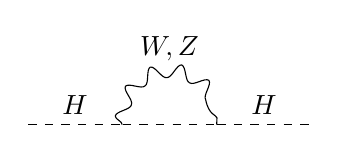
\begin{tikzpicture}[scale=1.2]
  \node[void] (in) at (0,0)  {};
  \node[void] (v1) at (1,0) {};
  \node[void] (v2) at (2,0) {};
  \node[void] (out) at (3,0) {};
  \draw[massvect] (v1) arc(180:0:0.5) ;
  \node at (1.5,0.8) {$W,Z$};
  \draw[spin0] (in) -- node [above]{$H$} (v1) -- (v2) -- node [above]{$H$} (out);
\end{tikzpicture}
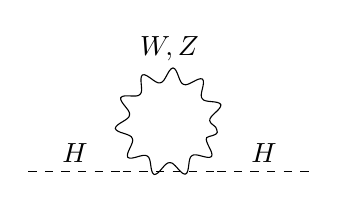
\begin{tikzpicture}[scale=1.2]
  \node[void] (in) at (0,0)  {};
  \node[void] (v1) at (1,0) {};
  \node[void] (v2) at (2,0) {};
  \node[void] (out) at (3,0) {};
  \draw[massvect] (1.5,0.45) circle (0.5);
  \node at (1.5,1.3) {$W,Z$};
  \draw[spin0] (in) -- node [above]{$H$} (v1) -- (v2) -- node [above]{$H$} (out);
\end{tikzpicture}
\begin{tikzpicture}[scale=1.2]
  \node[void] (in) at (0,0)  {};
  \node[void] (v1) at (1,0) {};
  \node[void] (v2) at (2,0) {};
  \node[void] (out) at (3,0) {};
  \draw[spin0] (1.5,0.5) circle (0.5);
  \node at (1.5,1.3) {$H$};
  \draw[spin0] (in) -- node [above]{$H$} (v1) -- (v2) -- node [above]{$H$} (out);
\end{tikzpicture}
\caption{One-loop quantum corrections to the Higgs boson mass. From left to right: contribution
from the Yukawa interaction; two contributions from the gauge interaction; contribution from the
Higgs self-interaction.
\label{fig:oneloopdiagrams}}
\end{figure}

A way to remove this quadratic dependence on the cutoff scale is to introduce extra particles in
the theory, with properties such that the loop behaviour is opposite to the Standard Model
particles. It is straightforward to show that we can cancel the fermionic loops by introducing
extra scalar particles. 
Assuming that there are $N_S$ new scalar particles, with mass $m_S$, trilinear coupling $v\lambda_S$
and quadrilinear coupling $\lambda_S$, we find as additional contribution to the
one-loop correction to the Higgs mass:
\begin{equation}
  \Delta m_H^2 =  \frac{N_S\lambda_S}{16\pi^2} \left[ - \Lambda^2 + 2 m_S^2 \log
\left(\frac{\Lambda}{m_S}\right)\right] - \frac{\lambda_S^2 N_S}{16 \pi^2} v^2 \left[ -1 + 2
\log\left(\frac{\Lambda}{m_S}\right) \right] + \mathcal{O}\left(\frac{1}{\Lambda^2}\right) .
\end{equation}
By assuming $\lambda_f^2 = - \lambda_S$ and $N_S = 2 N_f$, we find upon adding both
contributions, and using Eq.~\ref{eq:fermion_masses},
\begin{equation}
  \Delta m_H^2 = \frac{\lambda_f^2 N_f}{4\pi^2} \left[ \left(m_f^2-m_S^2\right)
\log\left(\frac{\Lambda}{m_S}\right) + 3 m_f^2 \log\left(\frac{m_S}{m_f}\right) \right] .
\end{equation}
All quadratically divergent terms have vanished. Introducing scalar particles with the
appropriate couplings has thus technically solved the hierarchy and naturalness problem. 
If in addition $m_S = m_f$, then the logarithmically divergent terms vanish as well. 

The divergencies introduced by the other loop diagrams in Fig.~\ref{fig:oneloopdiagrams} can also be
resolved by the introduction of new particles, fermions in this case, that have just the right
couplings to the Higgs boson. In this way all divergent contributions to the Higgs mass will
vanish, and no large finetuning is needed. 
%As we will see shortly, supersymmetry introduces extra particles that behave exactly in this
%way. 


\section{Extensions of the Standard Model \label{sec:extensions_standard_model}}


In an attempt to address some of the afore-mentioned open questions, numerous models of
beyond-the-SM (BSM) physics have been developed. With the discovery of the Higgs boson, some of
these are now ruled out~\cite{Cheng:2007bu}. Examples are the Higgsless models such as the most
basic incarnation of technicolour, or the models which predict a very large Higgs boson mass, such
as certain Composite Higgs models where the Higgs mass would be related to some new strong dynamics
at high scales. 
Nevertheless, several viable models still remain. A subset of these are presented in the following
sections.

\subsection{Supersymmetry \label{sec:supersymmetry}}

Supersymmetric models impose a new symmetry, supersymmetry (SUSY), that relates fermions and
bosons. Given that the razor boost analysis was developed with supersymmetry in mind and provides
interpretations in a SUSY context, I will discuss supersymmetric models in a separate chapter
(Chapter~\ref{chap:supersymmetry}) and only provide a brief motivation here. 

One of the nice features of SUSY is that it provides a solution to the hierarchy problem. 
The reason is that each known SM particle comes with a supersymmetric partner that differs in
spin by 1/2, and has the same mass. The structure of the couplings is also exactly as we suggested
in Section~\ref{sec:hierarchy_problem}, resulting in the removal of the quadratically divergent
terms in the mass correction. In practice we have not observed any such partner particles. Hence,
their masses cannot be equal to the corresponding SM particles, and SUSY must be broken somehow. 
If the breaking mechanism is such that the quadratic divergencies still cancel, but not necessarily
the logarithmic ones, then the hierarchy problem can still be solved. 

SUSY also triggers electroweak symmetry breaking in a dynamic way. There is thus no need to
explicitly assume a negative $\mu^2$ in the Higgs potential. 
A very generic SUSY Lagrangian would allow interactions leading to proton decay. To avoid this,
R-parity is introduced. If R-parity is conserved, then the lightest supersymmetric particle (LSP) is
stable, as it cannot decay without violating R-parity. This LSP can be a dark matter candidate, as
it would be heavy and only weakly interacting. 

For all these reasons, and more, SUSY is nowadays by far the most popular extension of the Standard
Model. Hopes are high to find hints of the existence of supersymmetric particles during the
upcoming Run 2 of the LHC. 

\subsection{Little Higgs scenarios \label{sec:little_higgs}}

In Little Higgs theories~\cite{Cheng:2007bu,Reuter:2012sd,Schmaltz:2005ky} the electroweak scale is
stabilized in a natural way. 
The Higgs boson is viewed as a pseudo-Goldstone boson of a new global symmetry that is broken,
both spontaneously and explicitly, by new physics around the 10\TeV scale. 
The Lagrangian contains two sets of interactions that explicitly break the symmetry, in addition to
the symmetric part $\mathcal{L}_0$
\begin{equation}
  \mathcal{L} = \mathcal{L}_0 + \lambda_1 \mathcal{L}_1 + \lambda_2 \mathcal{L}_2 .
\end{equation}
The Higgs boson would be an exact massless Goldstone boson if both couplings $\lambda_1$ and
$\lambda_2$ vanish, and can only acquire a mass if both of them are present. This means that
the corrections to the Higgs mass are suppressed by two loops w.r.t. the cutoff scale, and as such
the hierarchy problem only appears around a scale of 10\TeV, compared to 1\TeV for the SM. 
Similarly to supersymmetry, new particles are postulated to exist, but they should have the same 
spin as the known SM particles. 
Many choices for the new global symmetry can be made, resulting in slightly different model
predictions. To avoid having a big impact on electroweak precision observables, T-parity is usually
introduced. This parity ensures that the new particles have to be produced in pairs, as is the case
for R-parity in SUSY, which means they only impact the observables at loop-level. 

\subsection{Extra dimensions \label{sec:extra_dimensions}}

A key assumption in models of extra spatial dimensions~\cite{ArkaniHamed:1998rs}, is that the
electroweak scale is the only fundamental short distance scale. The loop corrections to the Higgs
mass are thus cut off at the electroweak rather than the Planck scale, resulting in a much less
finetuned model.  
The weakness of gravity is explained by assuming that gravity permeates these new dimensions, while
the gauge interactions do not. 
The Planck scale in ($4+n$) dimensions is assumed to be of the order of the electroweak scale.  
The effective Planck scale at large distances (larger than the size $R$ of the extra dimensions)
then becomes $M_{\text{Pl}(4+n)}\cdot R^n$. For $n\geq 2$, the needed size of the extra dimensions
is sub-millimetre, a scale where the current understanding of gravity has not been tested yet. 
Models of extra dimensions can be tested in the high-energy collisions at the
LHC~\cite{Chatrchyan:2011fq}. One could detect excited gravitons, which preferentially decay to two
high energy photons, or one could look for missing energy when particles disappear into the extra
dimensions. 


\chapter{Supersymmetry \label{chap:supersymmetry}}



\section{Simplified model spectra \label{sec:sms}}

% explain basics of simplified models


\chapter{The Large Hadron Collider and the Compact Muon Solenoid experiment \label{chap:LHC_CMS}}
\chaptermark{The LHC and the CMS experiment}

The analysis presented in this thesis uses $\Pp\Pp$ collision data delivered by the Large Hadron
Collider (LHC) and recorded by the Compact Muon Solenoid (CMS) experiment. An overview of the
collider is given in Section~\ref{chap:LHC}, while the detector setup is discussed in
Section~\ref{chap:CMS}.

\chapter{The Large Hadron Collider \label{chap:LHC}}


% briefly discuss


\chapter{The Compact Muon Solenoid experiment \label{chap:CMS}}

% briefly discuss each subsystem

% also mention trigger and data acquisition
% HLT refs \cite{Adam:2005zf,Agostino:2009nva}

\section{Trigger and data acquisition}

\subsection{L1 Trigger}

\subsection{HLT Trigger \label{sec:cms_hlt}}

% refer to next chapter for event reconstruction

\chapter[Event generation, simulation, reconstruction]{Event generation, simulation and
reconstruction \label{chap:event_generation}}

In the previous two chapters I discussed how $\Pp\Pp$ collisions are produced by the LHC, and
how they are detected by CMS. This chapter will elaborate on the different
steps needed to actually use the collisions for physics analysis. 
First I will explain more details about the collisions, or \textit{events}, themselves. I will
discuss the separate components an event consists of, as well as touch upon how events are described
mathematically. 

In order to understand what we observe in the data, which might contain signals of new physics, it
is important to know how Standard Model processes will appear in the detector. To achieve this we
generate those processes using Monte Carlo generation techniques, incorporating everything that is
known about how the Standard Model works. The principal options that are available to generate
events will be discussed in Section~\ref{sec:event_generation}. 
For each generated collision, we obtain a set of final state particles according to the specified
physics process. This could for example be the particles that result from the production and decay
of a top quark. 
At this stage we do not know yet how these particles would interact with the detector. That is
taken care of in a next step by the event simulation, as explained in
Section~\ref{sec:event_simulation}. An event simulator mimics how a particle, e.g. an electron,
would interact with all the different detector layers, and stores the response of the detector in
the same format as the actual detector data. 

At this point the simulated data and the real data are very similar, but are stored in a raw format,
containing detector hits and energy depositions, rather than physics objects. This format is hard to
use for further analysis. The final step will thus be to perform the event reconstruction. The
purpose of event reconstruction is to convert the raw detector information, be it real or simulated,
into physical objects, such as electrons, muons, photons, charged or neutral hadrons. Each of those
objects comes with a set of defining variables, which can be very basic (e.g. \pt, $\eta$ or $\phi$)
or more complex (e.g. shower shape). The different algorithms and techniques that are used within
CMS for this purpose are detailed in Section~\ref{sec:event_reconstruction}. 

\section{What is an ``event''? \label{sec:event}}

%%%%%%%%%%%%%%%%%%%%%%%%%%%%%%%%
%% What is an event? 
%%%%%%%%%%%%%%%%%%%%%%%%%%%%%%%%

At the LHC we define an \textit{event} as everything that happens in a proton bunch crossing.
These high energy collisions are very complex, often resulting in the production of many hundreds of
particles. An illustration of this complexity is shown in Fig.~\ref{fig:event_full_event}.
A proper description of what happens is impeded by the composite nature of the proton, and by the
strong coupling constant of QCD, the quantum field theory governing hadron
interactions.
Fortunately, it turns out that the full process can be factorized into independent subprocesses,
each taking place at different energy scales and, therefore, distance~\cite{Skands:2011pf}. 


\begin{figure}[p]
  \centering
  \includegraphics[width=0.98\textwidth]{figures/eventreco_event/full_event}
  \caption{Pictorial representation of a $\Pp\Pp$ collision event.
The hard interaction (big red blob) is followed by the decay of the produced particles (small red
blobs).
Additional hard QCD radiation is produced (red) and a secondary interaction takes place (purple
blob) before the final-state partons hadronize (light green blobs) and hadrons decay (dark green
blobs). Photon radiation occurs at any stage (yellow). Figure taken from
Ref.~\cite{Gleisberg:2008ta}
  \label{fig:event_full_event}}
\end{figure}


The process that is usually of most interest is the interaction between the constituents of the two
protons that results in high \pt particles. This is referred to as the \textit{hard interaction}. 
Not every collision produces very hard particles, sometimes protons merely undergo elastic
collisions, resulting in very soft scattering products that do not pass the detection thresholds. In
general, any interaction producing some detectable particles is called a \textit{minimum bias
interaction}~\cite{Field:2012jv}. 

The initial momentum distribution of the partons involved in the hard interaction is described by
\textit{parton distribution functions} (PDF). 
Apart from the hard interaction, the other constituents of the proton can also interact. This
usually results in a spray of softer particles, the \textit{underlying event} (UE). 
Any high momentum particle involved in the collision will emit QCD radiation.
Radiation from particles before the hard interaction is called initial-state-radiation (ISR),
whereas radiation off particles produced in the collision is called final-state-radiation (FSR).

Quarks and gluons produced in the collision cannot stay free; they must hadronize in a time scale
of $\mathcal{O}(\text{10}^{\text{-23}}\second)$. These hadrons, in addition to possible produced
leptons, will then pass through the experiment where they can be detected, and used to find out
what happened in the collision itself. 
A complication for the physicists analyzing the data arises from the very high
instantaneous luminosity at the LHC. During one bunch crossing there are usually up to 20
$\Pp\Pp$ interactions, collectively referred to as \textit{pileup}. Most of these interactions
produce relatively soft particles, but they do add to the overall hadronic activity in an event,
and can obscure the interesting hard process. 
An example of how an event might look like in the CMS detector is shown in
Fig.~\ref{fig:event_display}. 

In the next subsections I will elaborate on how to describe an event in a more mathematical way,
starting from the factorization theorem. These sections are largely based on
Refs.~\cite{Campbell:2006wx,Skands:2011pf,Salam_Bautzen,Salam:2010zt,Tung:2001cv}.

\begin{figure}[p]
  \centering
  \includegraphics[width=0.9\textwidth]{figures/eventreco_event/event_display_SUS12024}
  \caption{CMS event display showing five high \pt jets, three of which are tagged as coming from a
$\cPqb$ quark. Figure from~\cite{SUS12024_event_display}.
  \label{fig:event_display}}
\end{figure}


\subsection{Factorization theorems}

The basic problem addressed by factorization theorems~\cite{Collins:1989gx} is how to calculate
cross sections for high energy processes. In general, these cross sections are a combination of
short- and long-distance contributions, and are thus not computable directly using perturbation
theory.
Factorization theorems allow us to derive predictions for these cross sections,
by separating (factorizing) long-distance from short-distance effects. 
The long-distance effects, which cannot be described using perturbation theory - and therefore
referred to as “non-perturbative” effects, 
are encapsulated in parton distribution functions
describing the momentum distribution of partons in a hadron. 
These functions cannot be computed from first principles. Therefore, their form must be extracted
from data by comparing the predictions and measurements of suitable observables, see
Section~\ref{sec:event_pdfs}. Most importantly, the same functions can be used for different
processes for which the factorization theorem holds.
The short-distance hard-scattering cross section can be calculated with perturbation theory
because the QCD coupling strength is small at short distances. 

The factorization theorem applied to the cross section $\sigma$ of a hard scattering initiated by
two hadrons $A$ and $B$, illustrated in Fig.~\ref{fig:event_hard_scatter},
can be expressed in terms of the parton distribution functions $f$, and partonic cross section
$\hat{\sigma}$:
\begin{multline}
  \sigma(s;\alpha_S,\mu_F,\mu_R) = \\ 
  \sum_{a,b} \int_0^1 dx_a \int_0^1 dx_b \,  f_{a/A}(x_a, \alpha_S, \mu_F) \cdot f_{b/B}(x_b,
\alpha_S, \mu_F) \cdot \hat{\sigma}(\hat{s};\alpha_S,\mu_F,\mu_R),
\label{eq:factorization_theorem} 
\end{multline}
 \begin{wrapfigure}{r}{0.4\textwidth}
  \centering
  \vspace{-1eM}
  \includegraphics[width=0.38\textwidth]{figures/eventreco_event/Hardscattering}
  \caption{Diagram of a hard scattering process, showing the parton distribution functions
$f$ and the partonic cross section $\hat{\sigma}$. Figure taken from Ref.~\cite{Campbell:2006wx}.
  \label{fig:event_hard_scatter}}
\end{wrapfigure}
with $f_{a/A}(x_a, \alpha_S, \mu_F)$ the probability that a parton $a$ inside
a hadron $A$ carries a momentum fraction $x_a$, where $s$ is the centre-of-mass energy of the
collision, and $\hat{s} = s x_a x_b$ the partonic centre-of-mass energy.
The strong coupling constant is denoted by $\alpha_S$, the factorization scale by $\mu_F$ and the
 renormalization scale by $\mu_R$.
The factorization scale defines the (arbitrary) boundary between what is viewed as a short-distance
versus a long-distance interaction. The renormalization scale is also an arbitrary scale, which is
needed to regulate the divergencies that appear when computing the partonic cross section in a
perturbative expansion. 
Often, the choice $\mu_F = \mu_R$ is made for convenience.
Obviously, the physical cross section cannot possibly depend on these scales, which are artifacts of
calculations. Therefore, we expect an accurate prediction of the cross section to be insensitive to
these scales. However, when making computations,
%The left-hand side of the equation is in reality independent of the arbitrary choices for $\mu_F$
%and $\mu_R$. When making computations, 
a dependence can be introduced because we cannot
compute the partonic cross sections up to all orders in $\alpha_S$. 

The validity of this factorization theorem can be proven mathematically for certain classes of
processes (it is only approximately true for many other processes), but can also be understood
intuitively in the context of the parton model. 
Hadrons are viewed as composite objects, made up of partons held together by their interactions in
a virtual partonic state.
Let's consider how a hadron-hadron scattering at high energy and momentum transfer looks like in the
centre-of-mass frame. The hadrons appear Lorentz contracted in the direction of the collision, and
their internal interactions are time dilated. The higher the centre-of-mass energy, the longer the
lifetime of any virtual partonic state will be, and the shorter the time needed for a parton of one
hadron to cross the other hadron. At high enough energy, the time needed to traverse the hadron
will be much shorter than the lifetime of any partonic state. Each parton inside the hadron can
thus be viewed as carrying a definite fraction $\xi$ of the hadron's momentum in the centre-of-mass
frame, and so it makes sense to talk about the partons interacting rather than the hadrons.  
Therefore, the interactions of the partons inside a hadron, which occur at time-dilated time
scales before or after the hard scattering, cannot interfere with the interaction of a parton
from one hadron with a parton from the other hadron. 
The cross section for hadron scattering may thus be computed by
combining probabilities, rather than amplitudes, and factorization is reached. 




\subsection{Parton distribution functions \label{sec:event_pdfs}}

A key ingredient to the computation of any cross section at the LHC, is the set of parton
distribution functions describing the momentum distributions of partons within the proton, as
is visible from Eq.~\ref{eq:factorization_theorem}. 
Physically, PDFs express the fact that hadrons are composite objects, with a time-dependent
structure. The PDFs themselves are not physical observables, but rather a more fundamental quantity
derived from the actual physical observables such as structure functions, which can be measured
in e.g. deep-inelastic scattering processes. 
Parton distribution functions can be extracted from this data, but only within a specific
factorization scheme, order by order in perturbation theory. 
At leading order they have a very simple physical interpretation: if the PDF for a given particle
species $p$ is given by $p(x,Q^2)$, then $p(x,Q^2) dx$ is the probability that a probe of
virtuality $Q^2$ will find a particle of flavour $p$ inside the proton, with a
momentum fraction between $x$ and $x + dx$ of the full proton momentum. 
At higher orders, the PDFs no longer have a clear probabilistic interpretation. 

Parton distribution functions satisfy sum rules, governed by the valence content of the
hadrons. For a proton we find for the PDFs of the $u$, $d$,
and $s$ (anti)quarks: 
\begin{align}
  \int_0^1 dx \left( u(x,Q^2) - \bar{u}(x,Q^2)\right) &= 2, \\[-2pt]
  \int_0^1 dx \left( d(x,Q^2) - \bar{d}(x,Q^2)\right) &= 1, %\\[-2pt]
%  \int_0^1 dx \left( s(x,Q^2) - \bar{s}(x,Q^2)\right) &= 0, 
\end{align}
\begin{equation}
%  \int_0^1 dx \left( u(x,Q^2) - \bar{u}(x,Q^2)\right) &= 2, \\[-2pt]
%  \int_0^1 dx \left( d(x,Q^2) - \bar{d}(x,Q^2)\right) &= 1, \\[-2pt]
  \int_0^1 dx \left( s(x,Q^2) - \bar{s}(x,Q^2)\right) = 0, 
\end{equation}
while we also need the momentum weighted sum of the PDFs of all particle species to sum to unity, in
order to satisfy momentum conservation, 
\begin{equation}
  \int_0^1 dx \, x \left( g(x,Q^2) + \sum_i [u_i(x,Q^2) + \bar{u}_i(x,Q^2)]\right) = 1 ,
\end{equation}
where $g(x,Q^2)$ is the gluon PDF, and $i$ runs over all quark flavours. 

Looking back to Eq.~\ref{eq:factorization_theorem}, we note that the parton distribution
functions depend on the chosen factorization scale. The dependence of the PDFs on the scale $Q^2$
is described by the DGLAP equations, which can be viewed as renormalization group equations in
analogy with those for the running coupling constant. 
The DGLAP equations, and thus the PDF evolution, are governed by the so-called splitting functions,
$P_{ab}$ , that model the rate for a particle of type $a$ to undergo a collinear splitting to
produce a particle of type $b$. 

Parton distribution functions are obtained from global fits to a wide variety of data from
many experiments, among which are measurements of deep-inelastic scattering at HERA, and Drell-Yan
or inclusive jet production at the Tevatron and the LHC. 
Since there is only a partial kinematic overlap between these data and the region in $(x,Q^2)$ space
where we want to use the PDFs, for example to model the production of supersymmetric particles,
the DGLAP evolution is essential for the successful prediction of PDFs in the LHC domain. 
The splitting functions are now known up to NNLO precision, which reduced the uncertainties in the
evolution dramatically, from 30\% down to about 2\%.

As illustration of the PDF scale dependence, we show in Fig.~\ref{fig:NNPDF} the full
set of parton distribution functions for two $Q^2$ scales, as derived by the \textsc{NNPDF}
collaboration~\cite{Ball:2012cx}. 
The gluon PDF is seen to dominate for small momentum fractions, and this domination increases as the
scale increases. This simply means that as we probe the proton with higher energy, i.e. to smaller
length scales, we will find more and more gluons. 

\begin{figure}[tpb]
  \centering
  \includegraphics[width=0.8\textwidth]{figures/eventreco_event/nnpdf23_nnlo_allpdfs}
  \caption{Parton distribution functions for different parton species inside the proton for two
values for the momentum transfer, as obtained by the \textsc{NNPDF}
collaboration~\cite{NNPDF_website,Ball:2012cx}. 
  \label{fig:NNPDF}}
\end{figure}

Most global analyses, such as the one performed by the \textsc{CTEQ} or \textsc{MSTW}
collaborations, use a generic form for the parameterization of the quark and gluon distributions at
some reference value $Q_0$, usually chosen in the range $1-2\GeV$:
\begin{equation}
  f(x,Q_0) = A_0 x^{A_1} (1-x)^{A_2} P(x; A_3, \ldots) .
\end{equation}
The parameter $A_1$ is associated with small-$x$ behaviour, while $A_2$ is associated with
large $x$. These two factors are, in general, not sufficient to describe the quark or gluon
distribution functions. The term $P(x; A_3, \ldots)$ is a smooth function, depending on one or more
parameters, that is introduced to add more flexibility to the PDF parameterization. The various PDF
collaborations usually make different choices for the form of $P(x)$. 
The coefficients $A_i$ are then usually determined by comparing theoretical predictions with the
data using $\chi^2$ fits. 
The \textsc{NNPDF} collaboration uses a different approach, and parameterizes $f(x,Q_0)$ by a
neural network. 
Once the PDFs are determined for the reference value $Q_0$, they are generated for the full
$(x,Q^2)$ plane using the DGLAP evolution equations. 

Apart from having an estimate for the nominal values of the PDFs in a given kinematic range, it is
also important to understand the uncertainties, especially for the gluon PDF, which is the hardest
to access experimentally, and is constrained mostly by the $Q^2$ evolution of the quark PDFs. 
A common method of estimating parton distribution uncertainties is to compare different published
parton distributions. This poses a problem since most published PDF sets adopt similar
assumptions such that the differences between these sets do not fully capture the uncertainties that
actually exist. Several techniques exists that remedy this, and they are used by the PDF
collaborations to publish a proper set of uncertainties with each PDF set.  



\subsection{Hard interaction \label{sec:event_hard_interaction}}

% mention following things:
% - complications arising from MPI
% - make link to section on matrix element generators which will contain more info on the practical
% implementation


The partonic scattering cross section describes the hard interaction, and contains all the
short-range effects. For the interaction between two partons $a$ and $b$, resulting in final state
$F$ plus anything else ($X$), it can be written as
\begin{equation}
  \hat{\sigma}_{ab\rightarrow F+X} = \frac{1}{2\hat{s}_{ab}} | \mathcal{M}_{ab\rightarrow
F+X}|^2(\Phi_F, \mu_F, \mu_R), 
\end{equation}
with $\hat{s} = (p_a + p_b)^2$ the usual Mandelstam variable, and 
$|\mathcal{M}|^2$ the matrix element squared for the process $a b \rightarrow F+X$, appropriately
summed and averaged over the relevant helicities and colours. 
The matrix element depends on the final state phase space $\Phi_F$, and should be evaluated at the
factorization scale $\mu_F$ and renormalization scale $\mu_R$.

The partonic cross section can be expanded in a perturbative series in the strength of the
QCD coupling constant $\alpha_S$, 
\begin{equation}
  \hat{\sigma} = \hat{\sigma}_0 + \hat{\sigma}_1 \alpha_S + \hat{\sigma}_2 \alpha_S^2 + \ldots
\end{equation}
The first couple of terms in the perturbative expansion are the terms that so-called
\textit{fixed-order predictions} deal with. They are conceptually quite simple; it is easy to state
which contributions are included, and by including further orders in the expansion one can expect to
see improvement in the accuracy of the predictions. 
At leading order we can still compute many inclusive cross sections by hand, although this is often
automated, by computing all the relevant tree-level Feynman diagrams and integrating over the
appropriate phase space. 
At next-to-leading order we can distinguish between two sets of extra contributions to the
originally considered process: the real emissions resulting in extra quarks or gluons in the final
state, and the virtual loops which do not change the number of final state particles, but do impact
the cross section. 

It is important to note that the complexity of the computations increases mostly with the number of
extra loops, rather than the actual order in $\alpha_S$. 
Tree-level diagrams can be calculated up to quite high final-state multiplicities, $\sim\,$10,
while one-loop diagrams have only been used for processes with up to 3 or sometimes 4 final-state
particles, and two-loop diagrams are available only for $2 \rightarrow 1$ type processes, such as
$\Pp\Pp \rightarrow W$.
When going to higher orders in the perturbative series, it also becomes more and more tricky to
properly combine, i.e. cancel, divergencies between 2-loops, 1-loop and tree-level diagrams. 
Examples of tree-level diagrams that become divergent is anything produced in association with
extra quarks or gluons which could become soft or collinear. These divergencies must be cancelled
by the corresponding loop divergencies, otherwise unitarity is violated. 
In practice this is not always easy to do, especially when experimental cuts need to be applied. 
The standard technique to deal with this issue is through a \textit{subtraction procedure} which
introduces suitable counterterms, adding them to the real diagrams, and subtracting them from the
loops, hereby removing the divergencies from the calculation.


Even though the switch from LO to NLO predictions introduces some technical complications, it is
still worthwhile to do so, where possible, because of the reduced uncertainties. 
At NLO, the dependence on the factorization and renormalization scales is much smaller, as this
relies on the missing higher order terms, which for NLO contain an extra factor $\alpha_S$, and are
thus smaller.

The strength of the NLO correction is often encapsulated in a so-called NLO k-factor, which is
defined as the ratio of the NLO cross section to the LO cross section. K-factors for many processes
can be as large as 1.5, much larger than the 10\% effect one would expect from considering only the
extra factor of $\alpha_S$. The reason for this is that the terms accompanying that factor of
$\alpha_S$ can be quite large. 
The calculated k-factors can vary for different kinematic regimes within the same process, so care
needs to be taken when attempting to scale a LO cross section obtained for some particular corner of
phase space. 


As explained in the introduction of this chapter, we also need to generate full events for
which we can simulate the detector response, rather than only computing inclusive cross sections.
This chain often starts by generating events for the hard process only, of course taking into
account the parton distribution functions as well. 
Until recently, event generators based on the perturbative calculation of matrix elements could only
generate events up to LO. 
With the release of \textsc{MG5\_aMC@NLO}~\cite{Alwall:2014hca}, the automated generation of events
at NLO precision is now possible for almost any Standard Model process.
More details on how this is done in practice are presented in
Section~\ref{sec:event_matrix_element_generators}.






\section{Event generation \label{sec:event_generation}}

%%%%%%%%%%%%%%%%%%%%%%%%%%%%
%% Event generation 
%%%%%%%%%%%%%%%%%%%%%%%%%%%%

% add info on Madgraph, pythia, jet matching etc

\subsection{Matrix element generators}

\subsection{Parton shower and hadronization}

\subsection{Jet matching}


\section{Event simulation \label{sec:event_simulation}}

%%%%%%%%%%%%%%%%%%%%%%%%%%%%
%% Event simulation
%%%%%%%%%%%%%%%%%%%%%%%%%%%%

Simulation of the CMS detector response is done in one of two ways: a `full' simulation
(FullSim) which is time-consuming but very accurate, or a `fast' simulation (FastSim), which is much
faster, but for which approximations have been made. The following subsections will explain the
basic concepts and use cases for both of these options. 

\subsection{CMS Full Simulation using Geant4 \label{subsec:fullsim}}

The purpose of the CMS full simulation~\cite{Banerjee:2007zz,Banerjee:2011zzc,Banerjee:2012ge} is to
provide a very accurate description of how particles interact with the CMS detector. These simulated
event samples can then be used to understand and demonstrate the power of analysis methods which
will later be applied to the real data. They can also be used to derive calibrations, efficiencies
and resolutions for high level physics objects in case the available data are not sufficient

The inputs to the detector simulation are the hadronized particles from the event generator. These
particles and their four-vectors are passed to the simulation software in the \textsc{HepMC}
format~\cite{Dobbs:2001ck}. 
The particles are then propagated through the CMS detector using the \GEANTfour toolkit~\cite{G4}.
\GEANTfour contains a large collection of electromagnetic and hadronic physics processes describing
the interaction of particles with material, and the resulting energy loss. Examples of this are
bremsstrahlung, photon conversion, nuclear interactions, multiple scattering, and showering. In
case new particles are produced in these interactions, they are also propagated further. 

A key component for the success of the simulation is the precise implementation of the detector
geometry, material budget, and magnetic field strength. Not only the active layers need to be
accounted for, but also the cooling, cabling, and support structures. 
Choices must be made for the level of detail to include in the simulation geometry in order to
optimize computation speed versus the correctness of the simulation.
Within the CMS software framework there is a single, common implementation of the full detector
geometry for both the simulation and the reconstruction, ensuring full compatibility.

The accuracy of the detector implementation has been thoroughly tested with dedicated test beam
data, cosmic muon data, and early LHC collision data. Overall, very good agreement was
found, and adjustments were made where necessary. 

Pileup interactions are also added at this stage of the processing chain. A library of simulated
hits of minimum bias events is prepared beforehand, and then used to overlay a number of extra
interactions onto the signal event according to a specified pileup scenario. 
As the bunch crossing time is shorter than the time needed for particles of a given event to fully
traverse the CMS detector, we also need to take into account \textit{out-of-time pileup}, which is
the effect of previous or subsequent bunch-crossings on the current event. Out-of-time pileup is
modelled by modifying the timing of the detector hits when overlaying a minimum bias interaction. 

The next step is the conversion of all energy depositions, from signal and pileup events, in the
sensitive detector volumes to electronic signals. Electronic noise is also included during this
\textit{digitization} step.
The output of the digitization is simulated data in a format identical to that of real collision
data read directly from the detector. The L1 and HLT decisions, and the objects used to arrive at
them, are also included in the simulated data. 
From this point onwards the simulated events go through the same reconstruction steps as the real
data, as will be explained in Section~\ref{sec:event_reconstruction}. 





\subsection{CMS Fast Simulation \label{subsec:fastsim}}

% explain what approximations are made, why it is necessary, especially in SUSY searches


The CMS fast simulation~\cite{fastsim,Rahmat:2012fs} is a faster alternative to the full simulation
explained above. 
It is intended to be used for physics analyses that require the generation of many
samples to span a wide phase-space region, e.g. the vast SUSY simplified model scans. 
A set of approximations is made, resulting in a speed
increase of about a factor twenty. 

The interactions simulated in FastSim are electron bremsstrahlung, photon conversion, charged
particle energy loss by ionization, charged particle multiple scattering, nuclear interactions, and
electron, photon and hadron showering. The various CMS subsystems are modelled in different ways,
with various levels of approximation. 

The tracking detector is the most complicated CMS subsystem, and the one for which the most
approximations are made, including for the geometry.
The tracker is modelled by 30 thin nested cylinders, and is assumed to be made of pure silicon,
uniformly distributed over each layer. The thickness of each layer in terms of interaction lengths
was tuned to reproduce the number of bremsstrahlung photons above a certain threshold as observed in
FullSim.
Charged particles are propagated between two detector surfaces according to the magnetic field, and
experience multiple scattering and energy loss by ionization. The intersections between the
trajectories and each tracker layer define the position of the simulated hits that are then
converted into reconstructed hits with a certain efficiency, which is determined from FullSim. 

The showers of electrons and photons which hit the electromagnetic calori\-meter are simulated as if
the ECAL were a homogeneous medium. This is a reasonable approximation because the ECAL crystals
are organized to have almost no gaps in between them. 
Electrons and photons at rapidity values not covered by the electromagnetic calorimeter ($|\eta| >
3$) are propagated directly to the forward hadron calorimeter.

Charged and neutral hadrons are propagated to the start of the ECAL, HCAL and HF after their
interactions with the tracker layers. Their energy response is derived from the full
simulation. First the energy is smeared according to energy resolution measured in FullSim for
single pions. Then, this smeared energy is distributed in the calorimeters using parameterized
longitudinal shower profiles. 

Muons propagate through the tracker, the calorimeters, the solenoid, and the muon chambers. 
Both muons coming directly from the main interaction vertex and those produced inside the
tracker from the decay of another particle are included. 
The calorimeter response is treated similarly to that of charged hadrons. In the muon systems the
only processes that are taken into account are multiple scattering and energy loss by ionization.

The reconstruction of FastSim tracker hits into tracks is done in a different, faster, way compared
to FullSim or data. The truth information is used to group hits together that come from the same
particle. Consequently, FastSim does not have fake tracks. Two hits in the same place are also not
merged to be one reconstructed hit, as would be the case for the real detector readout. 
Despite these simplifications, good agreement between FastSim and FullSim track reconstruction is
observed. 





\section{Event reconstruction \label{sec:event_reconstruction}}

%%%%%%%%%%%%%%%%%%%%%%%%%%%
% Event reconstruction
%%%%%%%%%%%%%%%%%%%%%%%%%%%

The CMS event reconstruction aims to provide a global event description in terms of electrons,
muons, photons, charged hadrons, and neutral hadrons. Information from all subdetectors is combined
to achieve a fully consistent picture of the event. The algorithm that implements this, is called
particle flow (PF), and is documented in Refs.~\cite{CMS-PAS-PFT-09-001,PF}. 

Particle flow relies heavily on the high resolution sicilon tracker, and high granularity ECAL. The
basic building blocks are tracks, constructed using a very efficient tracking algorithm, and
clusters of calorimeter energy deposits. 
These two elements are then linked together using a linking algorithm. The actual particle flow
algorithm uses the links to create a list of reconstructed and identified particles, that are
subsequently used for physics analysis. A description of each of these steps will be given in
Section~\ref{sec:event_reco_pf}.

The particles that are reconstructed by the PF algorithm can be further refined to suit the needs
of individual analyses or analysis groups. More stringent identification criteria are usually
required, so that the misidentification rate, and thus background rate, is substantially reduced.
All physics objects that will be used in the razor boost analysis will be listed in
Section~\ref{sec:event_objects}.

Reconstructed events are sometimes affected by spurious detector noise or reconstruction failures,
leading to anomalous amounts of missing transverse momentum, or to very high \pt jets. 
These events are filtered out by various targeted cleaning algorithms, as discussed in
Section~\ref{sec:event_cleaning}.

The PF event reconstruction is applied in the same way to data and simulation, resulting in an
overall very good agreement between them. Some quantities cannot be adequately modelled in
simulation, however. Event reweighting techniques are employed to account for discrepancies that
might influence a physics analysis. In Section~\ref{sec:event_reweighting} I will discuss the
standard event reweighting techniques that are applied in the razor boost analysis. 


\subsection{Particle flow \label{sec:event_reco_pf}}


The particle flow method reconstructs particles, the PF candidates, by combining information from
the inner tracker, the calorimeters, and the muon system.  Each PF candidate is assigned to one of
five object categories: muons, electrons, photons, charged hadrons, and neutral hadrons.  

By simultaneously using information from all subdetectors, overlaps between object collections are
removed. In a calorimeter only reconstruction, for example, photons and electrons are also
reconstructed as jets. 
Since about 65\% of the jet energy is carried by charged hadrons, inclusion of the tracker
information in the jet reconstruction results in a much improved energy resolution. For jets
originating from a $\cPqb$ quark this is even more striking, as energy carried away by muons from
the $\cPqb$ decay can be included in the jet when taking a PF approach. 

The separate components of the PF algorithm are explained below, including a discussion on how
particle flow is used to suppress pileup effects.


\subsubsection{Iterative tracking}

The tracker provides a very good momentum resolution for charged hadrons, better than the
calorimeters up to a \pt of several hundred \GeV. It also gives a precise measurement of the
direction of charged particles. For these reasons, the tracker is the cornerstone of the PF
algorithm. A tracking efficiency as close to 100\% as possible, while keeping the tracking fake rate
as low as possible, is thus of the utmost importance.
An iterative, Kalman filter based, tracking strategy~\cite{Chatrchyan:2014fea} is used to achieve
this.

The track finding algorithm starts by requiring very tight criteria for the track seeds and
reconstruction quality, leading to a moderate tracking efficiency, but with a negligibly small fake
rate. 
The hits assigned to those tracks are then removed, and the tracking cycle is repeated two times
more for the remaining hits with progressively looser track seeding criteria. The looser criteria
increase the tracking efficiency, and the fake rate is kept low because of the reduced combinatorics
resulting from the removal of hits in the previous iteration. 
During three more iterations, the constraints on the origin vertex are also relaxed, allowing
the reconstruction of tracks associated with secondary vertices. 

With the iterative tracking technique, charged particles with a \pt as low as 150\MeV, as little
as three hits, and originating more than 50\unit{cm} from the beam axis, can be reconstructed with a
fake rate of the order of 1\%. 

\subsubsection{Calorimeter clustering}

The calorimeter clustering in the PF method aims for a high detection efficiency and a separation
of nearby energy deposits. 
The calorimeters are also solely responsible for providing a measurement of the energy and direction
of neutral hadrons and photons, and should provide additional information on charged hadrons in
case the track parameters could not be determined with high precision. 
The clustering is done separately for the ECAL, HCAL and preshower, and separately for barrel and
endcaps.
The algorithm consists of three steps. 
\begin{enumerate}
  \item Cluster seeds are identified as calorimeter cells with energy deposits above a certain
threshold, and larger than their neighbouring cells. 
  \item Topological clusters are grown from the cluster seeds by joining adjacent cells that pass a
chosen minimum energy threshold related to the level of noise in the electronics. 
  \item PF clusters are constructed from the topological clusters using an iterative procedure. Each
cluster seed gives rise to one PF cluster, even when multiple seeds are part of one large
topological cluster. If this happens, the energy of each calorimeter cell is shared among all PF
clusters according to the distance between cluster and cell. During the different iterations, the
PF cluster position is computed as a weighted average of the positions of the cells. As the
cluster position changes, the distance between cluster and cell changes, and thus the energy
sharing, which prompts the recalculation of the cluster position. This continues until the cluster
positions are stable. 
\end{enumerate}

% The purpose of a clustering algorithm in the calorimeters is at least fourfold:
% (ii) separate these neutral particles from energy deposits from charged hadrons; 
% (iii) reconstruct and identify electrons and all accompanying Bremsstrahlung photons; and 


\subsubsection{Link algorithm}

A particle passing through the CMS detector can leave hits in multiple subdetectors, as was
illustrated in Fig.~\ref{fig:cms_slice}, and will thus most likely give rise to multiple PF
elements. There can be a track, one or more calorimeter clusters, or possibly a track in the muon
system. The linking algorithm is designed to link together all elements originating from a single
particle, thereby removing any possible double counting from different subsystems. The quality of a
given link is quantified by the distance between the linked elements. 

A link between a charged particle track and a calorimeter cluster is made by extrapolating the
track to the calorimeters, at a depth corresponding to the expected shower maximum. The track is
linked to a calorimeter cluster if the extrapolated track position falls within the cluster. The
link distance is defined as the distance in the $(\eta,\phi)$ plane between the extrapolated track
position and the cluster position.  
Calorimeter clusters originating from bremsstrahlung photons emitted by electrons are captured by
extrapolating tangents to a track at each intersection between the track and a tracker layer
toward the ECAL. If the extrapolated tangent position is within a cluster, the cluster is linked to
the track as well.

Links between calorimeter clusters are made when the position of a cluster in the higher granularity
calorimeter falls within the boundaries of a cluster in the less granular calorimeter. The link
distance is defined as before. 

A charged-particle track in the tracker and a muon track in the muon system are linked when a global
fit between the two tracks returns an acceptable $\chi^2$, the value of which is used as link
distance. When several of these `global muons' can be fit using a given muon track and several
tracker tracks, only the global muon that returns the smallest $\chi^2$ is retained. 


\subsubsection{Particle reconstruction and identification}

The blocks of linked elements are converted into a set of identified particles by the particle-flow
algorithm. The order of the particle reconstruction follows how clean the signature is. Muons are
reconstructed first, neutral hadrons last. The full particle reconstruction and identification
algorithm proceeds in this way for each block of linked tracks and clusters. 

\begin{enumerate}
  \item Each global muon is added to the list of PF muons if its momentum is compatible with the
momentum determined using tracker information only. The track is then removed from the block. 

  \item The algorithm then proceeds to reconstruct electrons, using a dedicated
method~\cite{Khachatryan:2015hwa}. A Gaussian-Sum Filter is used to refit the candidate electron
track, taking into account the possible energy loss by bremsstrahlung, and follow its trajectory to
the ECAL. Seeds for the time-consuming fitting procedure are chosen only from the subset of tracks
that pass certain identification criteria.
An electron is fully identified if its track matches with an ECAL cluster, and if it passes a set of
tracking and calorimeter requirements. The electron is then added to the PF electron
collection, and the associated electron track and ECAL clusters, including those from
bremsstrahlung, are removed from the block before further processing. 

  \item The remaining tracks are subject to tighter quality criteria, namely the relative
uncertainty on the transverse momentum should be smaller than the relative calorimeter energy
resolution for charged hadrons. The presence of photons and neutral hadrons will be inferred from a
detailed comparison of the track momenta and calorimeter energies. 

  \item For each HCAL cluster all associated charged hadron candidate tracks are found. If a track
traverses more than one HCAL cluster, it is assigned to the closest one. 
  The charged hadron candidate tracks associated with a given HCAL cluster are then matched with
the ECAL clusters. The closest ECAL cluster they traverse is assigned to the charged hadron
candidate. If the track passes through multiple ECAL clusters, those clusters are first ordered by
distance. They are added, one by one, to the charged hadron candidate for as long as the total
calorimetric energy is smaller than the momentum of the charged particle track. 

  \item If the total reconstructed calorimeter energy is significantly smaller than the total
charged particle momentum, there is an inconsistency, and a relaxed muon reconstruction is
performed.
Tracks that fail more stringent track quality criteria are subsequently removed as well. 

  \item If on the other hand the total track momentum is smaller than the total calorimeter energy,
then the remaining tracks are indeed consistent with stemming from charged hadrons. The tracks are
thus added to the list of PF charged hadrons, with the track momentum as charged hadron momentum.

  \item For cases where the track momentum is compatible with the calorimeter energy, the charged
hadron energy and momentum are refit, using both tracker and calorimeter information. This is of
particular interest for high \pt hadrons, where the calorimeters provide a better resolution. 
 
  \item When there is a substantial excess of calorimeter energy compared to the track momentum,
photons and possibly neutral hadrons are reconstructed. First, photons are reconstructed from the
ECAL clusters. If this cannot account for the full excess, neutral hadrons are reconstructed from
the remainder.  
 
  \item Finally, ECAL and HCAL clusters without matching tracks are reconstructed as photons and
neutral hadrons, respectively. 
\end{enumerate}

At the end of the PF sequence, we now have a list of identified particles which can be used to
reconstruct jets. The user can specify which particle types are included in the jet reconstruction. 
By default, isolated muons and electrons are not included.  


\subsubsection{Pileup mitigation techniques}

The presence of pileup causes extra energy deposits and tracks to be overlaid with those of the
hard interaction. This results in a degraded resolution, and less clean signatures.
Pileup vertices are usually separated in space from the vertex of interest. The very precise
tracker system allows these vertices to be reconstructed, and we can use the particle flow
framework to mitigate the effect of in-time pileup, using a technique called \textit{charged
hadron subtraction}~\cite{CMS-PAS-JME-14-001}, or also \texttt{PFNoPileUp}. 

Contamination from pileup events is reduced by discarding charged hadron PF candidates that are
associated to pileup vertices, prior to jet clustering and any further processing.   
The leading primary vertex of the event is the one with the largest value of $\sum
|\pt^{\mathrm{track}}|^2$. The pileup vertices are all other primary vertices for which the number
of degrees of freedom (d.o.f.) in the vertex fit is greater than four. 
Charged hadrons are assigned to a particular vertex according to the compatibility, expressed as
the $\chi^2/\mathrm{d.o.f.}$, of the track with the proto-vertex reconstructed without the
currently considered track. If $\chi^2/\mathrm{d.o.f.}<20$ for a given track-vertex combination,
the track is associated to that vertex. 
Charged hadron candidates with a track associated to a pileup vertex are removed. All other tracks,
even when not associated to a vertex, are retained. 

Since charged hadron subtraction relies on the tracker information, it can only be applied within
the tracker acceptance, $|\eta| < 2.5$. It has been shown that this technique is successful at
removing a large portion of pileup jets, in addition to removing a significant part of the pileup
contribution to jets from the hard interaction. This results in an improved energy and angular
resolution. 


% The average pileup energy due to neutral hadrons is computed
% event-by-event and subtracted from the energy when computing lepton isolation and jet energy.  The
% energy subtracted is  the average pileup energy per unit area (in $\Delta\eta \times \Delta\phi$)
% times the jet area~\cite{Fastjet1, Fastjet2}.




\subsection{Physics object identification \label{sec:event_objects}}

The event selection is an integral part of any physics analysis. It determines which events are
used, and thus what processes contribute to the data sample. This in turn drives how the
backgrounds are estimated, what the sensitivity will be, et cetera. 
An event selection is most easily described in terms of particles, e.g. two electrons, no muons, at
least four jets, as this is the closest to how we think about a given process.  
The particle flow technique described in the previous section is very compatible with this approach,
given that it reconstructs a fully consistent set of identified particles out of the detector hits. 
However, a more thorough selection of the PF objects is needed in order to ensure that their
behaviour is understood, and to ensure that the selected events are not dominated by
misidentified particles, or detector artefacts. 
The physics object groups (POG's) within the CMS Collaboration are in charge of providing general
recommendations on how to define each object. These recommendations are based on extensive studies,
and are applicable for most analyses, thus reducing the workload for the analysis teams.
In the following paragraphs all the standard objects that will be used in the razor boost analysis
are discussed.


%%%%%%%%%%%%%%%%%%%%%%%%%%%%%%%%%%%%%%%%%%%%%%%%%%%%%%%%%%%%%%%%%%%%%%%%%%%%%%%%%%%%%%%%%%%%%%%%%

%%%%%%%%%%%%%%%%%%%%%%%%%%%%%%%%%%%
%%  Object identification
%%%%%%%%%%%%%%%%%%%%%%%%%%%%%%%%%%%



% The average pileup energy due to neutral hadrons is computed
% event-by-event and subtracted from the energy when computing lepton isolation and jet energy.  The
% energy subtracted is  the average pileup energy per unit area (in $\Delta\eta \times \Delta\phi$)
% times the jet area~\cite{Fastjet1, Fastjet2}.
% this corrects energy and momentum, not substructure
% TODO: move to jet and lepton sections

% 
% Missing transverse energy, which is used in the calculation of the razor variable $\mr$, is 
% defined to be the negative sum of the transverse momenta of all the particle flow objects in an
% event.  Loosely identified and isolated electrons with $\pt > 5$~\GeV and $|\eta| < 2.5$ and muons
% with $\pt > 5$\GeV and $|\eta| < 2.4$ are used both to suppress backgrounds in our signal region
%and
% in the definition of the control regions.  A tight definition of isolated leptons (electrons with
% $\pt > 10$~\GeV and $|\eta| < 2.5$ and muons with $\pt > 10$~\GeV and $|\eta| < 2.4$) defines a
% control region enriched in $\cPZ \rightarrow \ell \ell $ events, from which we estimate the
% systematic uncertainty in the predicted number of $\cPZ \rightarrow \nu \nu$ events in the signal
% region. Any electron candidates with $1.44 < |\eta| < 1.57$ are rejected since the transition
%region
% between barrel and endcap calorimeters is less well-instrumented.
% In order to suppress the decays of taus and other leptons that fail the loose selection, events
%that
% have isolated tracks with $\pt > 10$\GeV and track-primary vertex distance along the beam
%direction
% $dz < 0.05$ are rejected.

\subsubsection{Primary vertices \label{sec:object_vertex}}

We require at least one {\it good} primary vertex to be reconstructed in each event. 
This vertex should be associated with at least four charged-particle tracks. It should also lie
within 24\cm of the origin of the CMS coordinate system along the beam direction, and within 2\cm
in the plane transverse to the beam. 
These requirements, translated to the CMS nomenclature, are summarized in
Table~\ref{tab:object_vertex}.
In case there are multiple good vertices, we choose the vertex with the highest value of $\sum
\pt^2$ of associated tracks to be the leading primary vertex in the event. This vertex is
taken as a reference to reconstruct the event, e.g. to perform the track subtraction for pileup
removal, for which we use the charged hadron subtraction algorithm, as explained before.

\begin{table}[htdp]
\caption{Vertex selection criteria. \label{tab:object_vertex}}
\begin{center}
\begin{tabular}{l l}
\toprule
\texttt{\small isFake()} & $= 0$ \\
\texttt{\small ndof()} & $> 4$ \\
\texttt{\small z()} & $< 24\cm$ \\
\texttt{\small position.Rho()} & $< 2\cm$ \\
\bottomrule
\end{tabular}
\end{center}
\end{table}


\subsubsection{Jets \label{sec:object_jets}}

Most analyses are interested primarily in the quarks and gluon produced in the hard interaction, or
in the decay of heavy particles, such as top quarks or $\W$ bosons. 
However, through the process of parton showering and hadronization, the few initial quarks and
gluons turn into a multitude of hadrons. 
Hadrons from a given initial quark or gluon can usually be found close together, they form a
\textit{jet}. The proper description of jets, and the jet definitions that are used to reconstruct
them, relies on two properties: infrared, and collinear safety~\cite{Salam:2009jx}.
It is important that a jet definition returns the same set of final jets regardless of whether a
parton underwent a collinear or soft splitting. If this is not the case, i.e. the jet definition is
infrared or collinear unsafe, then one finds that divergencies in the theoretical computation of
jet cross sections do not vanish. 

A jet definition comprises two parts: the jet algorithm that defines in which order particles are
grouped together, and the recombination scheme that defines how to combine the momenta of the
to-be-merged particles. 
For the latter, the most common choice is to simply add the four-vectors of the particles, which
then gives rise to massive jets. 
For the jet algorithm there are many choices. Here I will focus solely on the anti-$k_\textrm{T}$
algorithm~\cite{antikt}, which is the default jet algorithm used by CMS.
As for most sequential recombination algorithms, one defines distances $d_{ij}$ between particles
$i$ and $j$ (or pseudojets if particles have been combined before),  and distances $d_{iB}$ between
particle $i$ and the beam.
The distance measures are in this case given by
\begin{align}
  d_{ij} &= \min \left(\frac{1}{p_{\mathrm{T,i}}^2}, \frac{1}{p_{\mathrm{T,j}}^2}\right)
\frac{\Delta R_{ij}^2}{R^2}, \\
  d_{iB} &= \frac{1}{p_{\mathrm{T,i}}^2},
\end{align}
where $\Delta R_{ij}^2 = (y_i - y_j)^2 + (\phi_i - \phi_j)^2$ and $R$ is a tuneable parameter
determining the size of the jets. The rapidity $y$ of a particle is given by,
\begin{equation}
  y = \frac{1}{2} \ln{\frac{ E + p_z }{ E - p_z }} .
\end{equation}
The jet clustering proceeds by identifying the smallest of all distances. If it is a $d_{ij}$, we
recombine particles $i$ and $j$, while if it is $d_{iB}$, we move $i$ from the list of particles to
the list of final jets. All distances are then recalculated and the procedure is repeated until no
particles are left.
The anti-$k_\textrm{T}$ algorithm results in mostly circular jets, reminiscent of the older cone jet
algorithms that are no longer used because they are not infrared and collinear safe.

The input to the jet clustering are the PF candidates that pass the charged hadron subtraction. 
The clustering itself is done with the anti-$k_\textrm{T}$ algorithm with size parameter $R=0.5$
(AK5), as implemented in \textsc{FastJet 3.0.1}~\cite{Cacciari:2011ma}.
We apply the standard loose identification criteria to the resulting jets, as defined by the
requirements listed in Table~\ref{tab:object_jets}. 

Unfortunately, the calorimeter response to incident particles is not uniform. It it, therefore, not
straightforward to translate the measured jet energy to the true particle energy, which is what we
want to use to do our analysis. A set of jet energy scale corrections -- scalings of the
jet four-momentum depending on jet \pt, $\eta$ and flavour -- are applied to both data and
simulation in order to achieve a proper mapping to the particle level. The difference between the
reconstructed and particle-level jet energy is called the \textit{offset} in what follows.
Jet energy corrections within CMS are taken care of in a sequential way, each level of correction
taking care of a different effect~\cite{JEC}. 

First, the residual effect from pileup is removed using the so-called L1 corrections. The effects
of charged hadrons from in-time pileup have already been largely reduced by the charged hadron
subtraction method. The effect of neutral particles and out-of-time pileup is removed at this stage
using a slightly modified version of the \textit{jet area method}~\cite{Fastjet1,Fastjet2}.
This method uses the effective area of the jets, $A$, multiplied by the average energy density
in the event, $\rho$, to calculate the energy to be subtracted from the jets.
Both real and simulated jets are first corrected with a $\pt$, $\eta$, and number of primary
vertices dependent offset correction determined in simulation. For data events, an additional
data/simulation scale factor is derived from ZeroBias data to correct for remaining $\eta$ dependent
discrepancies.
Figure~\ref{fig:JEC_L1} shows the size of the energy offset between reconstructed and particle level
jets, before and after the L1 corrections have been applied. A clear reduction of the overall offset
is observed. 

\begin{figure}[tpb]
  \centering
  \includegraphics[width=0.4\textwidth]{figures/eventreco_objects/OffMeantnpuRef_BB_ak5pfchs}
  ~
  \includegraphics[width=0.4\textwidth]{figures/eventreco_objects/OffMeantnpuRef_BB_ak5pfchsl1}
  \caption{The offset shown on the $y$-axis in these plots is defined as the difference in
transverse momentum for a reconstructed jet with added pileup and the same jet without pileup.
The lefthand side shows the offset as a function of the generated \pt of a jet before the L1
corrections have been applied, and the righthand side shows the offset after pileup
corrections. Different markers represent different levels of pileup. Figures taken from
Ref.~\cite{JEC_plots}.
  \label{fig:JEC_L1}}
\end{figure}


The second level of corrections, the L2 Relative corrections, are designed to make the jet response
flat in $\eta$. Since the simulation of the detector response is very detailed, see
Section~\ref{sec:event_simulation}, the jet response is in fact very well modelled in simulation,
which is why it is used for the bulk of the jet energy corrections. 
MC truth information is used to correct a jet at arbitrary $\eta$ relative to a jet
in the central area ($|\eta|<1.3$). 

\begin{figure}[tpb]
  \centering
\includegraphics[width=0.6\textwidth]
{figures/eventreco_objects/CorrectionVsEta_Overview_TDR_ak5pfl1_L2L3}
  \caption{ The size of the L2 and L3 corrections as a function of jet $\eta$ for three reference
transverse momentum values: 30\GeV (white hollow circles), 100\GeV (red squares) and 300\GeV (blue
circles). Figure taken from Ref.~\cite{JEC_plots2}.
  \label{fig:JEC_L23}}
\end{figure}


Then the L3 Absolute corrections, which flatten the jet response with respect to \pt, are applied.
They are derived from simulation, and correct the jet energy back to the particle level, such that
on average the \pt of a reconstructed jet matches that of a jet clustered using generator level
particles,
\begin{equation}
  <\pt(\mathrm{reco})_{\mathrm{corr}}> {=} <\pt(\mathrm{gen})>
\end{equation}
These are the final corrections applied to jets from simulated events. 

Data events are further corrected by the L2L3 Residual jet energy scale corrections to take care of
the small differences between data and simulation. These corrections are \pt and $\eta$ dependent,
and only correct the relative energy scale. The absolute energy scale was found to be well modelled
in the simulation. A dedicated, data-driven approach is employed, using data samples of dijet,
$\gamma+$jet, and $\cPZ+$jet events. 

% TODO Add information on jet corrections and pileup subtraction


% The jets are corrected for pile-up effects in a two step process.  
% First charged hadron particle-flow candidates that have been associated with a pile-up vertex are
% removed from the list of particles to be clustered using the {\tt PFNoPileUp} algorithm.  
% The jets are then clustered and corrected for the L2 and L3 corrections, taking into
% account the charged-hadron removal. 
% The remaining PU energy is subtracted by applying the event-by-event quantity $\pi \rho (\Delta
% R)^2$, where $\Delta R$ is the jet size and $\rho$ is the average density from PU events, as
% computed by {\tt FastJet} using only neutral hadron particle-flow candidates.  

After all corrections are applied, jets are required to have $\pt > 30\GeV$ and $|\eta| < 2.4$.  

  






\begin{table}[htdp]
\caption{Jet selection criteria. \label{tab:object_jets}}
\begin{center}
\begin{tabular}{l l}
\toprule
\pt & $> 30\GeV$ \\
$|\eta|$ & $< 2.4$ \\
\midrule
\texttt{\small neutralHadronEnergyFraction()} & $< 0.99$ \\
\texttt{\small neutralEmEnergyFraction()} & $< 0.99$ \\
\texttt{\small nConstituents()} & $> 1$ \\
\texttt{\small chargedHadronEnergyFraction()} & $> 0$ \\
\texttt{\small chargedMultiplicity()} & $> 0$ \\
\texttt{\small chargedEmEnergyFraction()} & $< 0.99$ \\
\bottomrule
\end{tabular}
\end{center}
\end{table}

The AK5 jets defined here will be used for most aspects of the razor boost analysis, except for the
reconstruction of boosted hadronic $\W$-candidates. 
Section~\ref{sec:boost_wtag} provides details on the dedicated jet treatment that is used for $\W$
tagging.

\subsubsection{B-Tagging \label{sec:object_btag}}

Jets originating from the hadronization of $\cPqb$ quarks can be distinguished from other jets,
initiated by gluons or light flavor quarks, due to the long lifetime of the $\cPqb$ quark. 
The non-prompt decay of the $B$ hadrons results in a secondary vertex, displaced with respect to
the primary vertex of the hard interaction. 

% TODO add more info on b-tagging algorithm

The ability to distinguish $\cPqb$ jets is especially important for new physics searches. Many new
physics models are associated with production of third generation quarks, whereas this is more rare
in the standard model. For many searches $\cPqb$ jet tagging is an essential tool in suppressing
the background from multijet or vector boson production. 

In the razor boost analysis $\cPqb$ tagging will also be employed. We will use the combined
secondary vertex (CSV) algorithm at two working points~\cite{btag7TeV,btag8TeV,BTagWP}, which are
shown on Table~\ref{tab:object_btag}. 
The Loose working point (CSVL), corresponding to a misidentification rate of $\sim$10\% and
efficiency of $\sim$85\%, will be used to veto $\cPqb$ jets, whereas the Medium working point
(CSVM), corresponding to a misidentification rate of $\sim$1\% and a typical efficiency of
$\sim$70\% , is used to select $\cPqb$ jets. 

\begin{table}[htdp]
\caption{Working points for the combined secondary vertex $\cPqb$ jet tagger.
\label{tab:object_btag}}
\begin{center}
\begin{tabular}{l l}
\toprule
Working point & Discriminator value \\
\midrule
Medium & $> 0.679$ \\
Loose & $> 0.244$ \\
\bottomrule
\end{tabular}
\end{center}
\end{table}
% 
% As will be explained in section~\ref{sec:selection}, we define our signal and control regions
% based on the number of b-tagged jets. 
% As the b-tagged jet multiplicity distribution is not exactly the same in data as in simulation, we
% need to apply appropriate Data/MC scale factors to the simulation. These scalefactors and their
% prescription have been provided by the BTag POG \cite{BTagSF1,BTagSF2}. 
% Whenever an explicit selection based on the number of b-tagged jets is made, the btag scale
% factors are applied to the simulation. 
% For more detailed information on the scale factors and their associated uncertainties, we refer to
% section~\ref{sec:btag_uncertainties}. 

% TODO Decide where to put the scale factor information

\subsubsection{Muons \label{sec:object_muon}}

Muons are identified using two different working points, a loose selection and a tight selection,
both of which will be detailed below. 


% Currently we mainly use the loose definition in the analysis, both for vetoing, and for selecting
% single muon events for the control regions enriched in TTJets and WJets. The tight selection is
% only used to define a control region enriched in $Z\rightarrow ll$ events, from which we derive a
% systematic uncertainty on the predicted number of $Z\rightarrow\nu\nu$ events in our signal
% region.

The \textbf{loose muon selection} that will be employed was developed especially for events with a
large amount of hadronic activity, where the standard identification criteria were observed to lose
efficiency, resulting in less background suppression when vetoing the presence of muons. 
The details and performance of this optimized selection is documented in
Ref.~\cite{CMS-AN2011-498}. 
The main feature is the use of a so-called \textit{directional} isolation.
The isolation of a particle is a measure of how far it is from other activity in the detector. The
leptons we are interested in, those originating in the hard interaction, are usually separated from
other activity, e.g. jets. This is not the case for misidentified muons or for muons from the decay
of heavy-flavour jets. Directional isolation is designed to have a better rejection of leptons from
these heavy-flavour jet decays, and is defined as
\begin{equation}
\overrightarrow{\mathrm{ISO}}(R) \equiv \sum_{\Delta R_{i} < R} \delta_{i}^{2}\pt{}_{i} ,
\end{equation}
where the sum is over all other particles $i$ within $\Delta R_{i}<R$ of the muon direction,
and $\delta_{i}$ is the angle between particle $i$ and the $\pt$-weighted centroid position
($\delta_{c}$) of all such particles in $(\eta,\phi)$ space. That is, if $\Delta\phi_i$ and
$\Delta\eta_i$ are respectively the difference in $\phi$ and $\eta$ angles between particle $i$ and
the muon, then:
\begin{eqnarray*}
\vec{e}_{i} & \equiv & \frac{1}{\sqrt{\Delta\phi_{i}^{2}+\Delta\eta_{i}^{2}}}\left(\begin{array}{c}
\Delta\phi_{i},\\
\Delta\eta_{i}
\end{array}\right),\\
\vec{\delta}_{c} & = & \sum_{\Delta R_{i}<R}\pt{}_{i}\vec{e}_{i},\\
\delta_{i} & = &
\angle(\vec{\delta}_{c},\vec{e}_{i})=\arccos(\vec{\delta}_{c}\cdot\vec{e}_{i}/|\vec{\delta}_{c}|),
\end{eqnarray*}
where $\vec{e}_{i}$ is the unit vector specifying particle $i$'s relative location in $(\eta,\phi)$
space with respect to the considered muon, as illustrated in Fig.~\ref{fig:object_directional_iso}.
Because of the weighting by $\delta_{i}^{2}$, the value for the directional isolation tends to be
larger for muons that are near the jet core, e.g. in case of leptonic $\cPqb$ decays, compared to
the more convential isolation definition which does not use this weighting. 

\begin{figure}[htpb]
  \centering
  \includegraphics[width=0.8\textwidth]{figures/eventreco_objects/directional_iso_cartoon}
  \caption{Illustration of ingredients used in the computation of directional isolation for a prompt
muon, denoted by a star, near some particles from a jet, denoted by points, in the $(\eta,\phi)$
plane. For prompt leptons $\delta_i$ tends to be small, especially for the high-\pt particles near
the core of the jet. Figure taken from Ref.~\cite{CMS-AN2011-498}.
  \label{fig:object_directional_iso}}
\end{figure}

Apart from the isolation, the identication criteria themselves are also altered from the standard
Loose Muon ID from the POG in order to further optimize the muon identification in environments
with large hadronic activity. 
Loose muons are reconstructed using either the global muon algorithm or the tracker-only
algorithm. 
Global muons are required to pass the {\tt GlobalMuonPromptTight} quality criteria,
and to have at least two muon chambers containing segments uniquely matched to its inner track. 
Tracker-only muons are required to pass the {\tt TMLastStationTight} criteria, which require the
muon to have compatible hits in the last muon chamber. 
All selected muons are then required to pass the selection listed in
Table~\ref{tab:object_loosemuon}. 
Some aspects of the selection depend on the muon $\pt$ and $\eta$; these are summarized in
Table~\ref{tab:object_loosemuon_cuts}.

\begin{table}[p]
\caption{Loose muon definition. }
\begin{center}
{\small
\begin{tabular}{l l}
\toprule
\pt & $> 5\GeV$ \\
$|\eta|$ & $< 2.4$ \\
\midrule
\texttt{\footnotesize innerTrack().hitPattern().numberOfLostHits()} & $\leq 1$ if $\pt < 20\GeV$ \\
                                                      & $\leq 4$ if $\pt \geq 20\GeV$ \\
$|\texttt{\footnotesize innerTrack().dxy(vertex.position())}|$ & $\pt$- and $\eta$-dependent\\
$|\texttt{\footnotesize muonBestTrack().dz(vertex.position())}|$ & $\pt$- and $\eta$-dependent\\
\midrule
$\overrightarrow{\mathrm{ISO}}(R=0.2)$ & $\pt$- and $\eta$-dependent \\
\bottomrule
\end{tabular}
}
\end{center}
\label{tab:object_loosemuon}
\end{table}

\begin{table}[p]
\caption{Details of the $\pt$ dependent thresholds employed in the loose muon selection.}
\begin{center}
  \begin{tabular}{l cccccc }
      \toprule
      Muon $\pt$  & $d_{xy} (\cm)$ & $d_{xy} (\cm)$ & $d_z (\cm)$ & $d_z (\cm)$ &
$\overrightarrow{\mathrm{ISO}}(0.2)$ &
$\overrightarrow{\mathrm{ISO}}(0.2)$ \\
      (\GeV) & Barrel & Endcap & Barrel & Endcap & Barrel & Endcap \\
      \midrule
      0 - 5          & 0.052 & 0.037 & 0.054 & 0.076 & 1.5  & 2    \\
      5 - 10         & 0.041 & 0.018 & 0.042 & 0.082 & 3    & 2.5  \\
      10 - 25        & 0.029 & 0.013 & 0.028 & 0.098 & 7    & 7.5  \\
      15 - 20        & 0.014 & 0.015 & 0.034 & 0.1   & 10.5 & 9    \\
      20 - 40        & 0.021 & 0.021 & 1     & 0.1   & 15.5 & 13.5 \\
      40 - 80        & 0.04  & 0.2   & 1     & 1     & 32.5 & 19   \\
      80 - 140       & 0.1   & 0.2   & 1     & 1     & 54.5 & 37   \\
      140 - 200      & 0.1   & 0.2   & 1     & 1     & 87   & 65.5 \\
      \bottomrule
    \end{tabular}
\end{center}
\label{tab:object_loosemuon_cuts}
\end{table}

 
The \textbf{tight muon selection} follows the recommendation from the Muon POG~\cite{MuonID}.
In addition to the identification criteria, we also require the tight muon to be isolated. 
Here we do not use directional isolation, but rather the more standard particle-based relative
isolation. 
This isolation, denoted $I_\mu$, is calculated using the PF candidates in a cone of size $\Delta R =
0.4$ around the muon. Charged-hadron candidates associated with pileup vertexes are not taken into
account in the calculation of the isolation. However, they are used to estimate the remaining
contribution to the isolation coming from neutral hadrons associated with pileup. This contribution
is then subtracted. 
The isolation definition is given by:
\begin{equation}
I_\mu = \frac{I_{Charged} + I_{Neutral} + I_{\gamma} - \Delta\beta\cdot I_{Charged}^{PU}}
             {\pt^\mu} , 
\label{eqn:iso}
\end{equation}
where $I_{Charged}$, $I_{Neutral}$, and $I_{\gamma}$ are computed as the sum of the \pt of the
charged hadrons, neutral hadrons and photons, respectively, in a cone of size $\Delta R = 0.4$
around the muon. The parameter $\Delta\beta$ is set to 0.5, and $I_{Charged}^{PU}$ is the estimated
contribution from pileup computed as the sum of the \pt of the charged hadrons associated with
pileup vertices.
The tight muon isolation requirement is $I_\mu < 0.15$.
A summary of the tight muon selection can be found in Table~\ref{tab:object_tightmuon}. 

\begin{table}[p]
\caption{Tight muon definition. }
\begin{center}
{\small
\begin{tabular}{l l}
\toprule
\pt & $> 10\GeV$ \\
$|\eta|$ & $< 2.4$ \\
\midrule
\texttt{\footnotesize isPFMuon()} & $= 1$ \\
\texttt{\footnotesize isGlobalMuon()} & $= 1$ \\
\texttt{\footnotesize globalTrack().normalizedChi2()} & $< 10$ \\
\texttt{\footnotesize globalTrack().hitPattern().numberOfValidMuonHits()} & $> 0$ \\
\texttt{\footnotesize track().hitPattern().trackerLayersWithMeasurement()} & $> 5$ \\
\texttt{\footnotesize innerTrack().hitPattern().numberOfValidPixelHits()} & $> 0$ \\
\texttt{\footnotesize numberOfMatchedStations()} & $> 1$ \\
$|\texttt{\footnotesize innerTrack().dxy(vertex.position())}|$ & $< 0.2\cm$ \\
$|\texttt{\footnotesize muonBestTrack().dz(vertex.position())}|$ & $< 0.5\cm$ \\
\midrule
$I_\mu =$ [\texttt{\footnotesize pfIsolationR04().sumChargedHadronPt()}& \\
\hspace{0.9cm} $+$ max(0., \texttt{\footnotesize pfIsolationR04().sumNeutralHadronPt()}  & \\
\hspace{2.7cm} $+$ \texttt{\footnotesize pfIsolationR04().sumPhotonPt()}  & \\
\hspace{2.7cm} $-$ 0.5 $\cdot$ \texttt{\footnotesize pfIsolationR04().sumPUPt()}) & \\
\hspace{0.9cm} ] / \pt & $< 0.15$ \\ 
\bottomrule
\end{tabular}
}
\end{center}
\label{tab:object_tightmuon}
\end{table}

 

\subsubsection{Electrons \label{sec:object_electron}}

Similar to the muon selection, we identify electrons using two different working points, a loose
selection, and a tight selection. 

% Currently we mainly use the loose definition in the analysis, both for vetoing, and for selecting
% single electron events for the control regions enriched in TTJets and WJets. The tight selection
% is only used to define a control region enriched in $Z\rightarrow ll$ events, from which we
% derive a systematic uncertainty on the predicted number of $Z\rightarrow\nu\nu$ events in our
% signal region.


The \textbf{loose electron selection} uses directional isolation as described in the previous
section, and fully documented in Ref.~\cite{CMS-AN2011-498}. A summary of the complete
loose electron selection is given in Table~\ref{tab:object_looseelectron}, with the details of
the $\pt$- and $\eta$-dependent requirements listed in Table~\ref{tab:object_looseelectron_cuts}. 

\begin{table}[p]
  \caption{Loose electron definition.}
  \begin{center}
  {\small 
    \begin{tabular}{l l l l}
      \toprule
      & Condition & Barrel & Endcap \\
      \midrule
      \pt & & $ > 5 \GeV$ & $> 5\GeV$ \\
      $|\eta|$ & & $ < 1.442$ & $1.556 - 2.5$ \\
      \midrule
      \texttt{\footnotesize gsfTrack().numberOfLostHits()} & $\pt < 20\GeV$ & $= 0$ & $= 0$ \\
      \texttt{\footnotesize gsfTrack().hitPattern().numberOfValidPixelHits()} & $\pt < 10\GeV$ &
$\geq 2$ & $\geq 1$ \\
      $|\texttt{\footnotesize gsfTrack().dz(vertex.position())}|$ & & \multicolumn{2}{l}{$\pt$- and
$\eta$-dependent}\\
      \midrule
      $\overrightarrow{\mathrm{ISO}}(R=0.3)$, calculated from charged particles only & &
\multicolumn{2}{l}{$\pt$- and $\eta$-dependent} \\
      $\overrightarrow{\mathrm{ISO}}(R=0.2)$, barrel only, calculated using all particles & &
\multicolumn{2}{l}{$\pt$- and $\eta$-dependent} \\
      \bottomrule
    \end{tabular}
    }
  \end{center}
  \label{tab:object_looseelectron} 
\end{table}


\begin{table}[p]
  \caption{Details of the $\pt$ dependent thresholds employed in the loose electron selection.}
  \begin{center}
  \begin{tabular}{ l ccccc }
      \toprule
      Electron $\pt$ & $d_z (\cm)$ & $d_z (\cm)$ &
$\overrightarrow{\mathrm{ISO}}(0.3,\textrm{charged})$ &
$\overrightarrow{\mathrm{ISO}}(0.3,\textrm{charged})$ & $\overrightarrow{\mathrm{ISO}}(0.2)$ \\
      (\GeV) & Barrel & Endcap & Barrel & Endcap & Barrel \\
      \midrule
      0 - 5          & 0.03 & 0.09 & 0.5  & 0.5  & 2    \\
      5 - 10         & 0.05 & 0.09 & 1.5  & 2.5  & 4.25 \\
      10 - 25        & 0.05 & 0.09 & 4.5  & 6.5  & 8.75 \\
      15 - 20        & 0.05 & 0.11 & 7.5  & 9    & 11   \\
      20 - 40        & 0.2  & 1    & 10   & 10.5 & 20.8 \\
      40 - 80        & 1    & 1    & 18.5 & 18.5 & 200  \\
      80 - 140       & 1    & 1    & 44   & 66.5 & 200  \\
      140 - 200      & 1    & 1    & 81.5 & 70   & 200  \\
      \bottomrule
    \end{tabular}
  \end{center}
  \label{tab:object_looseelectron_cuts}
\end{table}

The \textbf{tight electron selection} is in accordance with the recommendations of the EGamma POG
\cite{ElectronID}. A summary of the selection can be found in table~\ref{tab:object_tightelectron}.
We also require to electron to be isolated. The isolation is calculated using the PF candidates in a
cone of size $\Delta R = 0.3$ around the electron, and then corrected with an estimate of the
median energy from pileup as calculated with the {\tt FastJet} algorithm in a similar way to the
jet corrections explained in Sec.~\ref{sec:object_jets}. We require that this corrected isolation,
relative to the $\pt$ of the electron is less than 0.15.

\begin{equation}
I_e = \frac{ I_{Charged} + \max(0, I_{NeutralHad} + I_{\gamma} - A \rho ) }{\pt^e}
\end{equation}

% TODO: add more info on the pileup correction

\begin{table}[p]
\caption{Tight electron definition. }
\begin{center}
{\small
\begin{tabular}{l l l}
\toprule
& Barrel & Endcap \\
\midrule
\pt & $> 10\GeV$ & $> 10\GeV$\\
$|\eta|$ & $< 1.442$ & $1.556 - 2.5$ \\
\midrule
$|$\texttt{\footnotesize deltaEtaSuperClusterTrackAtVtx()}$|$ & $< 0.004$ & $< 0.005$ \\
$|$\texttt{\footnotesize deltaPhiSuperClusterTrackAtVtx()}$|$ & $< 0.030$ & $< 0.020$ \\
\texttt{\footnotesize sigmaIetaIeta()} & $< 0.010$ & $< 0.030$ \\
\texttt{\footnotesize hadronicOverEm()} & $< 0.120$ & $< 0.100$ \\
1.0/\texttt{\footnotesize ecalEnergy()} - \texttt{\footnotesize eSuperClusterOverP()/ecalEnergy()} &
$< 0.050$ &
$< 0.050$ \\
\texttt{\footnotesize gsfTrack().trackerExpectedHitsInner().numberOfHits()} & $\le 0$ & $\le 0$ \\
\texttt{\footnotesize passConversionVeto()} & $= 1$ & $= 1$ \\
$|\texttt{\footnotesize innerTrack().dxy(vertex.position())}|$ & $< 0.02\cm$ & $< 0.02\cm$\\
$|\texttt{\footnotesize gsfTrack().dz(vertex.position())}|$ & $< 0.1\cm$ & $< 0.1\cm$ \\
\midrule
$I_e$ & $<0.15$ & $< 0.15$ \\
\bottomrule
\end{tabular}
}
\end{center}
\label{tab:object_tightelectron}
\end{table}


\subsubsection{Isolated tracks \label{sec:object_isolatedtrack}}

In order to suppress the decays of both taus and other leptons that do not pass the loose
selection, we can veto events for which an isolated track is present~\cite{CMS-AN2013-089}. 
Isolated tracks are selected from the charged PF candidates with $\pt > 10\GeV$ and
longitudional track-primary vertex distance of $d_z < 0.05\cm$. They are required to have a
relative isolation in a cone of $\Delta R = 0.3$ of less than 0.1. 
In the razor boost analysis the isolated track veto will only be applied in the hadronic event
selections, and not in the control regions which require the presence of a lepton. 

\begin{table}[htdp]
\caption{Isolated track selection. }
\begin{center}
\begin{tabular}{l l}
\toprule
\pt & $> 10\GeV$ \\
\midrule
\texttt{charge()} & $> 0$ \\
$d_z({\rm PV, track})$ & $< 0.05\cm$ \\
$I_{\textrm{track}_i} = \frac{\sum_{j \neq i} \pt{}_j }{ \pt{}_i }$ & $< 0.1$ \\
\bottomrule
\end{tabular}
\end{center}
\label{tab:isolatedtrack}
\end{table}

\subsubsection{Missing transverse momentum \label{sec:object_met}}

The missing transverse momentum, \ETm, associated with a given event is computed as the negative
vector sum of the transverse momentum of all PF candidates $i$,
\begin{equation}
  \ETm = - \sum_i \pt^i .
\end{equation}
The corrections to the jet energy scale discussed above are propagated to the \ETm as well. 
Within CMS this type of missing transverse momentum is know as type-1 corrected \ETm.

No explicit selection will be placed on \ETm in the razor boost analysis selection, although it is
used in the definition of the razor variable $\rsq$, to be introduced in
Section~\ref{sec:boost_razor}.




\subsection{Event cleaning \label{sec:event_cleaning}}

The full CMS data taking and event reconstruction proces is very intricate. Every now and then a
subdetector might not have behaved properly, or a reconstruction algorithm could have failed. 
Events affected by such failures need to be removed from the selection, as they can for example
create artificially high missing transverse momentum.
The following cleaning filters are applied:

\begin{itemize}
\item The {\tt EcalDeadCellTriggerPrimitiveFilter}, which removes events where dead cells in the
ECAL produce anomalous activity.
\item The {\tt hcalLaserEventFilter}, which removes events where the HCAL laser produces anomalous
activity.
\item The {\tt hcalLaserEventFilter2012}, 
\item The {\tt trackingFailureFilter}, which removes events where the tracking algorithm does not
perform properly.
\item The {\tt CSCTightHaloFilter}, which removes events contaminated by beam halo.
\item The {\tt HBHENoiseFilter}, which removes events featuring large hadronic calorimeter noise.
\item The {\tt eeBadScFilter}, which removes events featuring high amplitude anomalous pulses due
to bad ECAL super-crystals.
\item The {\tt trkPOGFilters}, which remove events due to track reconstruction anomalies, such as
events with partly aborted track reconstruction and events affected by the Strip Tracker coherent
noise.
\item The {\tt primaryVertexFilter}, which removes events that do not have a good primary vertex.
\item The {\tt noscrapingFilter}, which removes events with a large multiplicity of low quality
tracks.
\end{itemize}

More details on these filters can be found in Ref.~\cite{metfilters}. The {\tt CSCTightHaloFilter}
and {\tt HBHENoiseFilter} filters are not applied for simulated samples that are
passed through the fast CMS detector simulation because the necessary input collections are
not produced.

In addition to the standard filters listed above, we also use an extra cleaning selection designed
to remove events with spurious HCAL noise originating in the Hadron Outer Calorimeter (HO). 
Energy deposits in the HO are included in the computation of the missing transverse momentum using 
the particle flow algorithm (PFMET), but are not included in the missing transverse energy obtained
from calorimeter information only (CaloMET). 
A selection requiring no substantial discrepancy between PFMET and CaloMET is thus effective at
reducing the contribution of these noisy events. 

We reject events in which the PFMET vector $\VEtmiss(\textrm{PF})$ is flipped with
respect to the CaloMET vector $\VEtmiss(\textrm{CALO})$. 
To accomplish this we compute the absolute value of the difference in polar angle,
 $|\Delta\phi_{\textrm{PF,CALO}}|$, taken in the range $[0,2\pi[$, and defined as
\begin{align}
|\Delta\phi_{\textrm{PF,CALO}}| &= \min \left ( \phi^{\textrm{PF}} - \phi^{\textrm{CALO}},   2\pi -
\phi^{\textrm{PF}} + \phi^{\textrm{CALO}} \right) ,\\
&\textrm{with } \phi^{\textrm{PF}} = \textrm{arctan} \left( \frac{\ETm(\textrm{PF})|_y}
{\ETm(\textrm{PF})|_x} \right) , \\
&\textrm{and } \phi^{\textrm{CALO}} = \textrm{arctan}\left( \frac{\ETm(\textrm{CALO})|_y}
{\ETm(\textrm{CALO})|_x} \right) .
\end{align}
Events for which $|\Delta\phi_{\textrm{PF,CALO}}|$ falls in a 1 radian window centred around $\pi$
are removed. 
\begin{equation}
\bigl| |\Delta\phi_{\textrm{PF,CALO}}| - \pi \bigr| < 1
\label{eqn:dphicut}
\end{equation}


\subsection{Event reweighting \label{sec:event_reweighting}}

The generation and simulation of events are tuned to mimic the data. However, the complete data
taking conditions, in particular the pileup profile, are not fully known before data
taking starts. It is thus impossible to mimic the data in all aspects. 
In addition to this, the event generation itself is also not perfect. For example, event generators
can only compute physics processes up to maximally NLO precision, whereas data contains all orders. 

To correct for some of these imperfections, event reweighting prescriptions have been developed. 
In the next subsections I will cover the reweightings that correct for mismodelling of the pileup
distribution, the initial state radiation (ISR), and the top quark \pt spectrum for the
$t\bar{t}$ simulation.

%%%%%%%%%%%%%%%%%%%%%%%%%%%%%
%% Event reweighting 
%%%%%%%%%%%%%%%%%%%%%%%%%%%%%

\subsubsection{Pileup reweighting \label{sec:event_pileup}}

The distribution of the number of pileup interactions is different in data with respect to
simulation. Given that the number of pileup interactions can have an influence on various aspects of
the reconstruction, such as the identification of primary vertices or lepton isolation, 
the simulated events should be reweighted such that their pileup distribution matches that of
data~\cite{pileup_twiki}.

The pileup distribution in data is provided centrally by the Physics Validation Group for each
data taking period. This distribution depends on the total \Pp\Pp inelastic cross section, sometimes
referred to as the \textit{minbias} cross section~\cite{Field:2012jv}. 
In simulation, the pileup distribution is taken from truth information, through the variable
\texttt{trueNumInteractions}. 
The pileup weights are computed as the ratio of the normalized pileup distributions in data and
simulation, and should be applied to all simulated events.
The distribution of the pileup in data and simulation, and the corresponding pileup weight is
shown in Figure~\ref{fig:pileup_comparison}. 

\begin{figure}[htpb]
 \centering
 \includegraphics[width=0.48\textwidth]{figures/eventreco_reweighting/pileup_comparison}
 ~
 \includegraphics[width=0.48\textwidth]{figures/eventreco_reweighting/pileup_weight_comparison}
\caption{[left] Comparison of the distribution of the true number of interactions in data and in
simulation. 
[right] Pileup weight as a function of the number of interactions. 
\label{fig:pileup_comparison}}
\end{figure}

% TODO decide whether to add the data mc comparison for the primary vertices

% 
% As a test of the performance of the pileup reweighting, we can check the agreement between data
% and
% simulation for the distribution of the number of good primary vertices ($PV$) at different
% selection
% levels. 
% We expect to find a reasonable, although not perfect agreement as the vertex reconstruction
% efficiency depends on many things. 
% This comparison is shown in figure~\ref{fig:comparison_PV}. 
% 
% \begin{figure}
%  \includegraphics[width=0.49\textwidth]{figures/Pileup/DataMC_PV_0Lb1Ll}
%  \includegraphics[width=0.49\textwidth]{figures/Pileup/DataMC_PV_g1Mb1Ll}
% \caption{Data/MC comparison plot of the number of good primary vertices after pileup reweighting
% for
% a control region enhanced in $W+$jets (left) and enhanced in $t\bar{t}+$jets (right).
% \label{fig:comparison_PV}}
% \end{figure}
% 


\subsubsection{ISR reweighting \label{sec:event_ISRreweighting}}

Searches for new physics often rely on an initial state boost of the produced system in order to
have experimental acceptance for the signature under consideration. This is especially important
for models featuring a compressed mass spectrum. A high-\pt ISR jet can be used to suppress
background, or the boost can raise the momentum of jets or leptons in the decay chain to a level
that is detectable.
A mismodelling of the initial state radiation, or uncertainty on the modelling, will thus
directly impact the interpretation of these searches. 

A study was performed to investigate how well the ISR is
modelled~\cite{Chatrchyan:2013xna,ISRreweighting} by evaluating the agreement between data and
simulation in the boost \pt for $\cPZ+$jets and $t\bar{t}$ events. 
For $\cPZ+$jets events the boost \pt was measured from the leptonic decay products of the $\cPZ$
boson. For $t\bar{t}$ events the ISR radiation was measured using the hadronic recoil system, which
is computed from all jets except for the $\cPqb$-tagged jets from the $t\bar{t}$ decay. 

It was found that the initial state radiation is not well modelled at high \pt. The mismodelling
can be corrected by applying a scale factor, with associated uncertainty, which was derived from the
observed disagreement. The scale factor depends on the \pt of the system recoiling against the ISR
jets. This system could be e.g. the $t\bar{t}$ system, the $\cPZ$ boson, or the $\tilde{g}\tilde{g}$
system for a SUSY event.  The uncertainty on this scale factor is taken to be the difference
between the scale factor and unity. 
The CMS SUSY group recommendeds to apply this ISR reweighting to all SUSY signal samples.
The prescription is summarized in Table~\ref{tab:ISRreweighting}. 

\begin{table}[htpb]
\caption{ISR reweighting prescription \label{tab:ISRreweighting}}
\begin{center}
\begin{tabular}{c c}
\toprule
\pt of recoiling & Scale factor \\ 
system (\GeV) & \\
\midrule
$\leq 120$ & $1.00 \pm 0.00$ \\
$120 - 150 $ & $0.95 \pm 0.05$ \\
$150-250$ & $0.90 \pm 0.10$ \\
$> 250$ & $0.80 \pm 0.20$ \\
\bottomrule
\end{tabular}
\end{center}
\end{table}

\subsubsection{Top quark \texorpdfstring{$\pt$}{pt} reweighting \label{sec:event_toppt_reweighting}}

Differential top-quark-pair cross section analyses have shown that the shape of the \pt spectrum of 
top quarks in data is softer than predicted by simulation~\cite{toppt,toppt_twiki}. 
To remedy this, events are reweighted based on the \pt of the generator level $t$ and $\bar{t}$
quarks in the $t\bar{t}$ simulation. 

The event weight, $w_{\rm TopPt}$, is computed as a function of the generated \pt of both the top
and anti-top quark
in the event: 
\begin{equation}
w_{\rm TopPt} = \sqrt{ SF_t \cdot SF_{\bar{t}} }
\end{equation}
\begin{equation}
SF(\pt^{gen}) = \exp(a + b\, \pt^{gen})
\end{equation}
with $a = 0.156$ and $b = -0.00137$.
The uncertainty associated with this reweighting is taken to be equal to the full size of the
reweighting, which gives for the up and down variations of the event weight:
\begin{align}
 +1~\sigma &: w_{\rm up} = w_{\textrm{TopPt}} * w_{\textrm{TopPt}}, \\
 -1~\sigma &: w_{\rm down} = 1 .
\end{align}

% 
% In figure~\ref{fig:TopPt} we show the Data/MC comparison for the $M_R$ and $R^2$ distribution in the
% $t\bar{t}+$jets control region (see section~\ref{sec:Tregion}) before and after applying the
% reweighting procedure. 
% We observe that this reweighting greatly improves the agreement between data and simulation. 
% Therefore we will always apply this reweighting to the $t\bar{t}+$jets simulated sample. 
% 
% \begin{figure}[htpb]
% \centering
% \includegraphics[width=0.49\textwidth]{
% figures/DataMC/DataMC_MR_g1Mbg1W1LlmT100_mdPhig0p5_width_noTopPt}
% \includegraphics[width=0.49\textwidth]{
% figures/DataMC/DataMC_R2_g1Mbg1W1LlmT100_mdPhig0p5_width_noTopPt}
% 
% \includegraphics[width=0.49\textwidth]{figures/DataMC/DataMC_MR_g1Mbg1W1LlmT100_mdPhig0p5_width}
% \includegraphics[width=0.49\textwidth]{figures/DataMC/DataMC_R2_g1Mbg1W1LlmT100_mdPhig0p5_width}
% \caption{[top] $M_R$ (left) and $R^2$ (right) distribution before applying the top \pt reweighting
%          [bottom] $M_R$ (left) and $R^2$ (right) distribution after applying the top \pt reweighting
% for the $T$ region as defined in section~\ref{sec:Tregion}
% \label{fig:TopPt}}
% \end{figure}
% 
% 
% 



\chapter{The razor boost analysis \label{chap:razorboost}}

In this chapter the razor boost analysis will be discussed. 
I will first cover the motivation and general strategy of the analysis in sections~\ref{sec:boost_motivation} and \ref{sec:boost_strategy}. 
Then the \textit{razor variables}, which are our most important discriminating variables, will be derived in section~\ref{sec:boost_razor}.
Section~\ref{sec:boost_wtag} details the technique used to tag highly boosted $\W$ bosons. 
The signal and control region selections are listed in sections~\ref{sec:boost_signal_selection} and \ref{sec:boost_control_selection}. 
The full statistical treatment, with its likelihood based approach, is explained in section~\ref{sec:boost_likelihood}. 
In section~\ref{sec:boost_systematics} the different sources of systematic uncertainties are discussed, followed by the results of the full
background estimation in section~\ref{sec:boost_results}. 
This chapter concludes, in section~\ref{sec:boost_interpretation}, with the interpretation of the results in terms of several simplified model spectra. 

\section{Motivation \label{sec:boost_motivation}}

% put text from note and expand. 
% use xkcd style plots
% look at emails from Harrison and Maurizio

\section{General strategy \label{sec:boost_strategy}}

% control regions, transfer factors
% binning in razor variables
% statistical treatment and systematic uncertainties

\section{Razor variables \label{sec:boost_razor}}

%%%%%%%%%%%%%%%%%%%
% razor variables
%%%%%%%%%%%%%%%%%%%

% add full derivation
% plots of signal and background

Many extensions of the Standard Model (see chapter~\ref{chap:beyond_standard_model}) predict the 
existence of new particles, which can be pair-produced in the proton-proton collisions at the LHC. 
Some of those theories introduce an extra symmetry, such as the R-parity in supersymmetry. A
consequence of this symmetry is that the lightest BSM particle must be stable, as it cannot decay
to SM particles only. This lightest BSM particle, called LSP in supersymmetric theories, is weakly
interacting, and escapes the detector unseen. 

This general property leads us to a generic class of new physics signatures in which a heavy
particle is pair-produced, and decays into visible, i.e. interacting with our detector, SM
particles, and an invisible LSP. This signature is illustrated in figure~\ref{fig:razor_signature}.

\begin{figure}[htpb]
  \centering
  %\includegraphics[width=0.5\textwidth]{} TODO add figure
  \caption{Generic new physics signature. Two massive new particles are produced in $\Pp\Pp$
collisions at the LHC, and consequently decay to a visible system and an invisible system. 
\label{fig:razor_signature}}
\end{figure}

Several kinematical variables targetting this topology have been developed.
% TODO add citations here
Most of these variables rely on the presence of the invisible LSP's. This causes the visible system
to deviate from a di-jet topology, resulting in possibly large missing transverse momentum, altered
angular distributions, et cetera. All of this can be used to distinguish the sought-after signal
from the known background processes. 
Unfortunately, the ultimate goal of reconstructing the masses of the new particles cannot be
attained. Because of the escaping LSP's, there is simply not enough information available to fully
constrain the problem. What we can do, however, is approximate the mass scale of the new physics
particles. Often times this results in variables that exhibit a kinematic edge. 
The \textit{razor variables} \cite{rogan,Rogan:1557072} are no exception in this regard. One
advantage the razor variables have over many other variables, is that they also reconstruct the
mass scale as a peak, in addition to a kinematic edge. 
In what follows I will derive the two razor variables, denoted \mr and \rsq, which use longitudinal
and transverse event information, respectively, to estimate a characteristic mass scale associated
with the new particles. At the end of this section I will briefly show how the razor variables are
used in the razor boost analysis. 

% explain reference frames

\subsection{Kinematical configuration and notation \label{sec:razor_notation}}

Let's again consider figure~\ref{fig:razor_signature}. For simplicity, we will assume that the
produced particles $S_1$ and $S_2$ undergo a two-body decay. Each $S_i$ decays to a visible,
standard model particle $Q_i$, and a particle $\chi_i$ that escapes the detector. 
We assume a symmetric decay chain, with the following relations for the masses of the different
particles,
\begin{alignat}{3}
  M_{S_1} &= M_{S_2} &&= M_S \label{eq:equal_S_masses}\\
  M_{\chi_1} &= M_{\chi_2} &&= M_{\chi} \label{eq:equal_chi_masses}\\
  M_{Q_1} &= M_{Q_2} &&= 0 \label{eq:no_Q_masses}
\end{alignat}

There are four relevant reference frames for our goal of determining a characteristic mass scale
of the new physics process under consideration. The following paragraphs will go through each of
these and define the notations that will be used, as well as deriving relations between several
variables. 

\paragraph{$S_1$ rest frame} 
From basic two-body decay kinematics it follows that the $Q_1$ and $\chi_1$ particles are produced
back to back, with equal magnitude of momentum, in the rest frame of the $S_1$ particle. This is
illustrated in figure~\ref{fig:razor_S1_rest_frame}. 

\begin{figure}[htpb]
  \centering
  %\includegraphics[width=0.6\textwidth]{×} % TODO make the figure
  \caption{Configuration of the $S_1$ rest frame. The decay products $Q_1$ and $\chi_1$ are
produced back to back with momenta $\vec{p}^S_1$ and $-\vec{p}^S_1$, respectively. 
\label{fig:razor_S1_rest_frame}}
\end{figure}

We can compute the magnitude of this momentum in terms of the new particle masses. To do this we
start from the four-vectors of the $Q_1$ and $\chi_1$ particles in the $S_1$ rest frame, 
\begin{alignat}{6}
  P[Q_1]    &\equiv q_1^S   &&= \{ E^S_{Q_1}, \vec{q}^S_1\} , \\
  P[\chi_1] &\equiv \nu_1^S &&= \{ E^S_{\chi_1}, \vec{\nu}^S_1\} .
\end{alignat}
Conservation of energy in the $S_1$ rest frame leads to 
\begin{equation}
  E^S_{Q_1} + E^S_{\chi_1} = M_S . \label{eq:razor_conservation_energy}
\end{equation}
This can also be expressed as
\begin{equation}
  \sqrt{M_{Q_1}^2 + (\vec{q}^S_1)^2 } + \sqrt{M_{\chi_1}^2 + (\vec{\nu}^S_1)^2} = M_S .
\end{equation}
Using Eq.~\ref{eq:equal_chi_masses} and Eq.~\ref{eq:no_Q_masses} (massless $Q_1$), and the equal
momenta $|\vec{q}^S_1| = |\vec{\nu}^S_1| = |\vec{p}^S_1|$, the above can be simplified as
\begin{align}
  |\vec{p}^S_1|   &= M_S - \sqrt{M_{\chi}^2 + (\vec{p}^S_1)^2} \\
  (\vec{p}^S_1)^2 &= M_S^2 - 2 M_S \sqrt{M_{\chi}^2 + (\vec{p}^S_1)^2} + M_{\chi}^2 +
(\vec{p}^S_1)^2 \\
  2 M_S \sqrt{M_{\chi}^2 + (\vec{p}^S_1)^2} &= M_S^2 + M_{\chi}^2 \\
  4 M_S^2 (\vec{p}^S_1)^2 &= (M_S^2)^2 + 2 M_S^2 M_{\chi}^2 + (M_{\chi}^2)^2 - 4 M_S^2
M_{\chi}^2 \\
  (\vec{p}^S_1)^2 &= \frac{(M_S^2 -M_{\chi}^2 )^2}{4 M_S^2} .
\end{align}

We thus find for the magnitude of the momentum of $Q_1$ and $\chi_1$ in the $S_1$ rest frame
\begin{equation}
  |\vec{p}^S_1| = \frac{M_S^2 -M_{\chi}^2}{2 M_S} \equiv \frac{M_\Delta}{2} ,
\label{eq:razor_p_S1_rest_frame}
\end{equation}
where we have defined the characteristic scale $M_\Delta$. This scale is exactly the scale we are
interested in. The goal of the \textbf{razor variables} is to \textbf{express $M_\Delta$ using lab
frame quantities only}. To succeed in this effort, we will have to make several, physics-motivated,
approximations. These will remove the unknown degrees of freedom, and are further explained in
sections~\ref{sec:razor_mr} and \ref{sec:razor_r2}. 

The energy of the $Q_1$ and $\chi_1$ particles can also be computed easily. 
From the masslessness of $Q_1$, we immediately find using Eq.~\ref{eq:razor_p_S1_rest_frame}
\begin{equation}
  E^S_{Q_1} = |\vec{p}^S_1| = \frac{M_\Delta}{2}. \label{eq:razor_E_Q1}
\end{equation}
To compute $E^S_{\chi_1}$, we substitute Eq.~\ref{eq:razor_E_Q1} in 
Eq.~\ref{eq:razor_conservation_energy}, and find 
\begin{align}
  E^S_{\chi_1} &= M_S - |\vec{p}^S_1|\\
	       &= M_S - \frac{M_S^2 -M_{\chi}^2}{2 M_S} \\
	       &= \frac{2M_S^2 - M_S^2 + M_{\chi}^2}{2 M_S} \\
	       &= \frac{M_S^2 + M_{\chi}^2}{2 M_S} \\
	       &= \frac{M_S^2 - M_{\chi}^2}{2 M_S} \frac{M_S^2 + M_{\chi}^2}{M_S^2 - M_{\chi}^2} .
%               &= \frac{M_\Delta}{2} R_{S\chi}
\end{align}

We can summarize the four-momenta of $Q_1$ and $\chi_1$ in the $S_1$ rest frame as
\begin{align}
  q_1^S   &= \frac{M_\Delta}{2} \{ 1, \vec{u}_1\} , \\  
  \nu_1^S &= \frac{M_\Delta}{2} \{ R_{S\chi}, -\vec{u}_1\} ,
\end{align}
with $$R_{S\chi} = \frac{M_S^2 + M_{\chi}^2}{M_S^2 - M_{\chi}^2},$$ and $\vec{u}_1$ the unit
vector along the $Q_1$ momentum direction.



\paragraph{$S_2$ rest frame}
The discussion of the $S_2$ rest frame is fully analogous to that of the $S_1$ rest frame. We
again find that
\begin{align}
  q_2^S   &= \frac{M_\Delta}{2} \{ 1, \vec{u}_2\} , \\  
  \nu_2^S &= \frac{M_\Delta}{2} \{ R_{S\chi}, -\vec{u}_2\} ,
\end{align}
and thus
\begin{equation}
  |\vec{p}^S_1| = |\vec{p}^S_2| = \frac{M_\Delta}{2} .
\end{equation}


\paragraph{Center-of-mass frame}
In the center-of-mass (CM) frame of the considered $\Pp\Pp$ collision events the particles $S_1$
and $S_2$ are produced with equal and opposite velocities $\betaCM$, as
illustrated in figure~\ref{fig:razor_CM_frame}. This is a consequence of
Eq.~\ref{eq:equal_S_masses}. 

\begin{figure}[htpb]
  \centering
  %\includegraphics[width=0.6\textwidth]{×} % TODO make the figure
  \caption{Configuration of the center-of-mass frame. The particles $S_1$ and $S_2$ are
produced back to back with velocities $\betaCM$ and $-\betaCM$, respectively. 
\label{fig:razor_CM_frame}}
\end{figure}

The four-vectors of particles $S_1$ and $S_2$ in the center-of-mass frame are given by
\begin{alignat}{6}
  P[S_1] &\equiv s^{\textrm{CM}}_1  &&= \{ E^{\textrm{CM}}_{S_1} , \vec{s}^{\textrm{CM}}_{S_1}\} 
&&= M_S \, \gamma^{\textrm{CM}} \, \{ 1 , \betaCM\} , \\ 
  P[S_2] &\equiv s^{\textrm{CM}}_2 &&= \{ E^{\textrm{CM}}_{S_2} , \vec{s}\,^{\textrm{CM}}_{S_2}\}
&&= M_S \, \gamma^{\textrm{CM}} \, \{ 1 , -\betaCM\}, \\ 
\end{alignat}
and satisfy the following
\begin{equation}
  (s^{\textrm{CM}}_1 + s^{\textrm{CM}}_1)^2 = \hat{s} = 4 (\gamma^{\textrm{CM}} M_S)^2,
\end{equation}
with $\sqrt{\hat{s}}$ the center-of-mass energy of the collision. 
To go from the rest frame of $S_1$ ($S_2$) to the CM frame, we need to boost the four-momenta
$q_1^S$ and $\nu_1^S$ ($q_2^S$ and $\nu_2^S$) to the frame travelling at velocity $\betaCM$
($-\betaCM$) with respect to the $S_1$ rest frame. 



\paragraph{Lab frame}


\subsection{Derivation of \mr \label{sec:razor_mr}}

\subsection{Derivation of \rsq \label{sec:razor_r2}}













% The razor variables \mr and \rsq \cite{rogan,Rogan:1557072} are useful for
% describing a signal due to pair production of heavy particles, each of which
% decays to a massless visible particle and a massive invisible particle. The signal will appear
% as a peak on a smooth exponentially falling SM background.  
% For this reason, the razor variables are robust discriminators for SUSY signals in which 
% supersymmetric particles are pair-produced and subsequently decay to SM particles and the LSP.  
% For the simple case in which the final state
% comprises two visible particles, e.g. jets, the razor variables are defined using the momenta 
% $\vec{p}_{{\rm j}_1}$ and $\vec{p}_{{\rm j}_2}$ of the two jets as
% \begin{eqnarray}
%  \label{eq:MRstar}
%  \mathrm{M_R} & \equiv &
%  \sqrt{
%    (|\vec{p}_{{\rm j}_1}|+|\vec{p}_{{\rm j}_2}|)^2 -
%    (p^{{\rm j}_1}_z+p^{{\rm j}_2}_z)^2}
%  \; ,\\
% %\end{eqnarray}
% %\begin{eqnarray}
%  \mathrm{M_T^{R}} & \equiv & \sqrt{ \frac{\ETm(p_T^{j1}+p_T^{j2}) -
%       \VEtmiss {\mathbf \cdot}
%       (\vec{p}_T^{\,j1}+\vec{p}_T^{\,j2})}{2}} \; ,
% \end{eqnarray}
% 
% where \VEtmiss is the missing transverse momentum vector in the event and \ETm is its magnitude.
% Given $\mathrm{M_R}$ and the transverse quantity $\mathrm{M^R_T}$, the razor dimensionless ratio is defined as
% \begin{eqnarray}
% \mathrm{R} \equiv \frac{\mathrm{M_T^R}}{\mathrm{M_R}}
% \; .
% \end{eqnarray}
% When the decay chains are complicated and therefore give rise to multiple particles in the final state,
% the razor variables can still be calculated by first reducing the final state to a two-``megajet'' structure.
% The megajet algorithm aims to cluster SM particles coming from the same heavy supersymmetric particle.  The
% razor variables \mr and \rsq are computed using the 4-momenta of the two megajets, where the megajet 4-momentum is the sum of the 4-momenta of the particles comprising  the megajet.  Studies show that of all possible clusterings the one that minimizes the sum of the invariant masses of the two megajets is the most efficient in assigning 
% correctly the particles to their heavy supersymmetric particle ancestor~\cite{razorPRL}. 



\section[Boosted W boson tagging]{Boosted $\W$ boson tagging \label{sec:boost_wtag}}

% explain n-subjettiness and jet pruning
% quote some plots and numbers from the JME PAS. 

\section{Signal region selection \label{sec:boost_signal_selection}}

\section{Control region selection \label{sec:boost_control_selection}}

\section{Statistical modelling \label{sec:boost_likelihood}}

% appendix on likelihoods and CLs?

\section{Systematic uncertainties \label{sec:boost_systematics}}

% add details on different sources
% add info on various extra studies

\section{Results \label{sec:boost_results}}

\section{Interpretation in terms of simplified model spectra \label{sec:boost_interpretation}}

% ref{sec:sms}


\chapter{Summary and outlook \label{chap:summary}}

...

% appendices
\appendix

\chapter{Data sets \label{app:datasets}}


\begin{sidewaystable}
\fontsize{8 pt}{1 em}
\selectfont
\caption{Simulated samples for the various background processes. The dataset names have been
stripped from /AODSIM.}
\begin{center}
\begin{tabular}{l l l l}
\toprule
Process & Dataset name & $\sigma$ (pb) & Level \\
\midrule
\multirow{2}{*}{$t\bar{t}$} &
/TTJets\_MassiveBinDECAY\_TuneZ2star\_8TeV-madgraph-tauola/Summer12\_DR53X-PU\_S10\_START53\_V7A-v1 
& 245.8 & NNLO \\
& /TTJets\_MassiveBinDECAY\_TuneZ2star\_8TeV-madgraph-tauola/Summer12-START53\_V7C\_FSIM-v2 & & \\
\midrule
QCD multijet, $100 < \HT< 250\GeV$ & 
/QCD\_HT-100To250\_TuneZ2star\_8TeV-madgraph-pythia/Summer12\_DR53X-PU\_S10\_START53\_V7A-v1
& 10.367$\times 10^{7}$ & LO \\
QCD multijet, $250 < \HT< 500\GeV$ &  
/QCD\_HT-250To500\_TuneZ2star\_8TeV-madgraph-pythia6/Summer12\_DR53X-PU\_S10\_START53\_V7A-v1
& 276000 & LO \\
QCD multijet, $500 < \HT< 1000\GeV$ & 
/QCD\_HT-500To1000\_TuneZ2star\_8TeV-madgraph-pythia6/Summer12\_DR53X-PU\_S10\_START53\_V7A-v1 
& 8426 & LO \\
QCD multijet, $\HT > 1000\GeV$ & 
/QCD\_HT-1000ToInf\_TuneZ2star\_8TeV-madgraph-pythia6/Summer12\_DR53X-PU\_S10\_START53\_V7A-v1 
& 204 & LO \\
\midrule
$\W\W$ & /WW\_TuneZ2star\_8TeV\_pythia6\_tauola/Summer12\_DR53X-PU\_S10\_START53\_V7A-v1 &
54.838 & LO \\
$\W\cPZ$ & /WZ\_TuneZ2star\_8TeV\_pythia6\_tauola/Summer12\_DR53X-PU\_S10\_START53\_V7A-v1 
& 32.3161 & LO \\
$\cPZ\cPZ$ & /ZZ\_TuneZ2star\_8TeV\_pythia6\_tauola/Summer12\_DR53X-PU\_S10\_START53\_V7A-v1
& 8.258 & LO \\
\midrule
$\W(\rightarrow\ell\nu)$+jets, $250 < \HT< 300\GeV$ & 
/WJetsToLNu\_HT-250To300\_8TeV-madgraph\_v2/Summer12\_DR53X-PU\_S10\_START53\_V7A-v1 & 48.01
& LO \\
$\W(\rightarrow\ell\nu)$+jets, $300 < \HT< 400\GeV$ &
/WJetsToLNu\_HT-300To400\_8TeV-madgraph\_v2/Summer12\_DR53X-PU\_S10\_START53\_V7A-v1 & 38.3 &
LO \\
$\W(\rightarrow\ell\nu)$+jets, $\HT > 400\GeV$ &
/WJetsToLNu\_HT-400Toinf\_8TeV-madgraph\_v2/Summer12\_DR53X-PU\_S10\_START53\_V7A-v1 & 25.22
& LO \\
\midrule
$t$, $t\W$-channel &
/T\_tW-channel-DR\_TuneZ2star\_8TeV-powheg-tauola/Summer12\_DR53X-PU\_S10\_START53\_V7A-v1 &
11.1 & NNLO \\
$\bar{t}$, $t\W$-channel &
/Tbar\_tW-channel-DR\_TuneZ2star\_8TeV-powheg-tauola/Summer12\_DR53X-PU\_S10\_START53\_V7A-v1
& 11.1 & NNLO \\
$t$, $s$-channel &
/T\_s-channel\_TuneZ2star\_8TeV-powheg-tauola/Summer12\_DR53X-PU\_S10\_START53\_V7A-v1 & 3.79
& NNLO \\
$\bar{t}$, $s$-channel &
/Tbar\_s-channel\_TuneZ2star\_8TeV-powheg-tauola/Summer12\_DR53X-PU\_S10\_START53\_V7A-v1 &
1.76 & NNLO \\
$t$, $t$-channel &
/T\_t-channel\_TuneZ2star\_8TeV-powheg-tauola/Summer12\_DR53X-PU\_S10\_START53\_V7A-v1 & 56.4
& NNLO \\
$\bar{t}$, $t$-channel &
/Tbar\_t-channel\_TuneZ2star\_8TeV-powheg-tauola/Summer12\_DR53X-PU\_S10\_START53\_V7A-v1 &
30.7 & NNLO \\
\midrule
$\cPZ (\rightarrow \nu \bar{\nu})$+jets, $50 < \HT < 100\GeV$ & 
/ZJetsToNuNu\_50\_HT\_100\_TuneZ2Star\_8TeV\_madgraph/Summer12\_DR53X-PU\_S10\_START53\_V7A-v1 
& 381.2 & LO \\
$\cPZ (\rightarrow \nu \bar{\nu})$+jets, $100 < \HT < 200\GeV$ &
/ZJetsToNuNu\_100\_HT\_200\_TuneZ2Star\_8TeV\_madgraph/Summer12\_DR53X-PU\_S10\_START53\_V7A-v1 
& 160.3 & LO \\
$\cPZ (\rightarrow \nu \bar{\nu})$+jets, $200 < \HT < 400\GeV$ &
/ZJetsToNuNu\_200\_HT\_400\_TuneZ2Star\_8TeV\_madgraph/Summer12\_DR53X-PU\_S10\_START53\_V7A-v1 
& 41.49 & LO \\
$\cPZ (\rightarrow \nu \bar{\nu})$+jets, $\HT > 400\GeV$ &
/ZJetsToNuNu\_400\_HT\_inf\_TuneZ2Star\_8TeV\_madgraph/Summer12\_DR53X-PU\_S10\_START53\_V7A-v1 
& 5.274 & LO \\
\midrule
$\cPZ/\gamma^* (\rightarrow \ell \bar{\ell})$+jets, $200 < \HT < 400\GeV$ &
/DYJetsToLL\_HT-200To400\_TuneZ2Star\_8TeV-madgraph/Summer12\_DR53X-PU\_S10\_START53\_V7A-v1
& 19.73 & LO \\
$\cPZ/\gamma^* (\rightarrow \ell \bar{\ell})$+jets, $\HT > 400\GeV$ &
/DYJetsToLL\_HT-400ToInf\_TuneZ2Star\_8TeV-madgraph/Summer12\_DR53X-PU\_S10\_START53\_V7A-v1
& 2.826 & LO \\
\midrule
$\W(\rightarrow q\bar{q})+bb$ & 
/Wbb\_FullyHadronic\_8TeV\_madgraph/Summer12\_DR53X-PU\_S10\_START53\_V7C-v1 & 121 & LO \\
$\cPZ/\gamma^*\rightarrow c\bar{c}$ & 
/DYToCC\_M\_50\_TuneZ2star\_8TeV\_pythia6/Summer12\_DR53X-PU\_S10\_START53\_V7A-v1 & 3060.099 & LO
\\
$\cPZ/\gamma^* \rightarrow \cPqb\bar{\cPqb}$ & 
/DYToBB\_M\_50\_TuneZ2star\_8TeV\_pythia6/Summer12\_DR53X-PU\_S10\_START53\_V7A-v1 & 3840.386 & LO
\\
\midrule
$\W\W\W$ & /WWW\_8TeV-aMCatNLO-herwig/Summer12\_DR53X-PU\_S10\_START53\_V7C-v1 & 0.08058 & NLO \\
$\W\W\cPZ$ & /WWZNoGstarJets\_8TeV-madgraph/Summer12\_DR53X-PU\_S10\_START53\_V7A-v1 & 0.05795 & NLO
\\
$\W\cPZ\cPZ$ & /WZZ\_8TeV-aMCatNLO-herwig/Summer12\_DR53X-PU\_S10\_START53\_V7C-v1 & 0.01968 & NLO
\\
$\cPZ\cPZ\cPZ$ & /ZZZNoGstarJets\_8TeV-madgraph/Summer12\_DR53X-PU\_S10\_START53\_V7A-v1 & 0.005527
& NLO \\
$\W\W\gamma$ & /WWGJets\_8TeV-madgraph\_v2/Summer12\_DR53X-PU\_S10\_START53\_V7A-v1 & 0.528 & LO \\
\midrule
$t\bar{t}\cPZ$ & /ttbarZ\_8TeV-Madspin\_aMCatNLO-herwig/Summer12\_DR53X-PU\_S10\_START53\_V19-v1 
& 0.2057 & NLO \\
$t\bar{t}\W$ & /TTbarW\_8TeV-aMCatNLO-herwig/Summer12\_DR53X-PU\_S10\_START53\_V7C-v1 & 0.232 & NLO
\\
$t\bar{t}\gamma$+jets & /TTGJets\_8TeV-madgraph/Summer12\_DR53X-PU\_S10\_START53\_V19-v1 & 1.44 & LO
\\
$t\bar{t}\W\W$+jets & /TTWWJets\_8TeV-madgraph/Summer12\_DR53X-PU\_S10\_START53\_V7A-v1 & 0.002037 &
LO \\
\bottomrule
\end{tabular}
\end{center}
\label{tab:boost_mc_bg}
\end{sidewaystable}

\begin{sidewaystable}
\fontsize{8 pt}{1 em}
\selectfont
\caption{MC simulated samples for the signal events.}
\begin{center}
\begin{tabular}{l l}
\toprule
Topology & Dataset name \\
\midrule
\multirow{10}{3.5cm}{T2tt \begin{align*}
pp \rightarrow\, &\stopone \stopone^*, \\[-3pt]
               &\stopone \rightarrow t \lsp \\[-3pt]
               \end{align*}} &
/SMS-T2tt\_mStop-150to350\_mLSP-0to250\_8TeV-Pythia6Z/Summer12-START52\_V9\_FSIM-v1 \\
& /SMS-T2tt\_mStop-375to475\_mLSP-0to375\_8TeV-Pythia6Z/Summer12-START52\_V9\_FSIM-v1 \\
& /SMS-T2tt\_mStop-500to650\_mLSP-0to225\_8TeV-Pythia6Z/Summer12-START52\_V9\_FSIM-v1 \\
& /SMS-T2tt\_mStop-500to650\_mLSP-250to550\_8TeV-Pythia6Z/Summer12-START52\_V9\_FSIM-v1 \\
& /SMS-T2tt\_mStop-675to800\_mLSP-0to275\_8TeV-Pythia6Z/Summer12-START52\_V9\_FSIM-v1 \\
& /SMS-T2tt\_mStop-675to800\_mLSP-300to700\_8TeV-Pythia6Z/Summer12-START52\_V9\_FSIM-v1 \\
& /SMS-8TeV-Pythia6Z\_T2tt\_mStop-150to475\_mLSP-1/Summer12-START52\_V9\_FSIM-v1 \\
& /SMS-8TeV-Pythia6Z\_T2tt\_mStop-500to800\_mLSP-1/Summer12-START52\_V9\_FSIM-v1 \\
& /SMS-T2tt\_mStop-825to900\_mLSP-1\_and\_mLSP-25to800\_8TeV-Pythia6Zstar/Summer12-START52\_V9\_FSIM-v3 \\
& /SMS-T2tt\_mStop-925to1000\_mLSP-1\_and\_mLSP-25to900\_8TeV-Pythia6Zstar/Summer12-START52\_V9\_FSIM-v3 \\
\midrule
\multirow{6}{3.5cm}{T1ttcc, fixed gluino mass 
\begin{alignat*}{3}
pp \rightarrow\, &\tilde{g} \tilde{g}, \\[-3pt]
               &\tilde{g} \rightarrow t &&\stopone, \\[-3pt]
               & &&\stopone \rightarrow c \lsp
\end{alignat*}}
&/SMS-MadGraph\_Pythia6Zstar\_8TeV\_T1ttcc\_2J\_mGo-1000\_mStop-310-325-350-375\_mLSP-300/Summer12-START52\_V9\_FSIM-v1 \\
&/SMS-MadGraph\_Pythia6Zstar\_8TeV\_T1ttcc\_2J\_mGo-1000\_mStop-410-425-450-475\_mLSP-400/Summer12-START52\_V9\_FSIM-v1 \\
&/SMS-MadGraph\_Pythia6Zstar\_8TeV\_T1ttcc\_2J\_mGo-1000\_mStop-510-525-550-575\_mLSP-500/Summer12-START52\_V9\_FSIM-v1 \\
&/SMS-MadGraph\_Pythia6Zstar\_8TeV\_T1ttcc\_2J\_mGo-1000\_mStop-610-625-650-675\_mLSP-600/Summer12-START52\_V9\_FSIM-v1 \\
&/SMS-MadGraph\_Pythia6Zstar\_8TeV\_T1ttcc\_2J\_mGo-1000\_mStop-710-725-750-775\_mLSP-700/Summer12-START52\_V9\_FSIM-v1 \\
&/SMS-MadGraph\_Pythia6Zstar\_8TeV\_T1ttcc\_2J\_mGo-1000\_mStop-810-825-850-875\_mLSP-800/Summer12-START52\_V9\_FSIM-v1 \\
\midrule
\multirow{6}{3.5cm}{T1ttcc, fixed $m_{\stopone} - m_{\lsp}$
\begin{alignat*}{3}
pp \rightarrow\, &\tilde{g} \tilde{g}, \\[-3pt]
                   &\tilde{g} \rightarrow t &&\stopone, \\[-3pt]
                   &                        &&\stopone \rightarrow c \lsp
\end{alignat*}}
&/SMS-T1ttcc\_2J\_mGo-600to750\_mLSP-1to500\_DM-10\_TuneZ2star\_8TeV-madgraph-tauola/Summer12-START53\_V19\_FSIM\_PU\_S12-v1 \\
&/SMS-T1ttcc\_2J\_mGo-600to750\_mLSP-1to500\_DM-25\_TuneZ2star\_8TeV-madgraph-tauola/Summer12-START53\_V19\_FSIM\_PU\_S12-v1 \\
&/SMS-T1ttcc\_2J\_mGo-600to750\_mLSP-1to500\_DM-80\_TuneZ2star\_8TeV-madgraph-tauola/Summer12-START53\_V19\_FSIM\_PU\_S12-v1 \\
&/SMS-T1ttcc\_2J\_mGo-800to1300\_mLSP-1to500\_DM-10\_TuneZ2star\_8TeV-madgraph-tauola/Summer12-START53\_V19\_FSIM\_PU\_S12-v1 \\
&/SMS-T1ttcc\_2J\_mGo-800to1300\_mLSP-1to500\_DM-25\_TuneZ2star\_8TeV-madgraph-tauola/Summer12-START53\_V19\_FSIM\_PU\_S12-v1 \\
&/SMS-T1ttcc\_2J\_mGo-800to1300\_mLSP-1to500\_DM-80\_TuneZ2star\_8TeV-madgraph-tauola/Summer12-START53\_V19\_FSIM\_PU\_S12-v1 \\
\midrule
\multirow{4}{3.5cm}{T1t1t
\vspace{-1.5ex}
\begin{alignat*}{3}
pp \rightarrow\, &\tilde{g} \tilde{g}, \\[-3pt]
                   &\tilde{g} \rightarrow t &&\stopone, \\[-3pt]
                   &                        &&\stopone \rightarrow t \lsp
\end{alignat*}}
&/SMS-T1t1t\_2J\_mGo-800to1300\_mLSP-1to500\_DM-175\_TuneZ2star\_8TeV-madgraph-tauola/Summer12-START53\_V19\_FSIM\_PU\_S12-v1 \\
&/SMS-T1t1t\_2J\_mGo-600to750\_mLSP-1to500\_DM-175\_TuneZ2star\_8TeV-madgraph-tauola/Summer12-START53\_V19\_FSIM\_PU\_S12-v1 \\
& \\
& \\
& \\
\bottomrule
\end{tabular}
\end{center}
\label{tab:boost_mc_sms}
\end{sidewaystable}


%
\chapter{CLs method \label{app:CLs}}

\textcolor{red}{TODO: Add CLs explanation here...}

\chapter[Systematic uncertainties for signal]{Systematic uncertainties across the T1ttcc
(\texorpdfstring{$\mathbf{\Delta m = 25}\GeV$}{Dm=25GeV}) mass plane 
\label{app:signal_systematics}}

In the section on systematic uncertainties, in Table~\ref{tab:bgsigsys}, we presented the average of
the systematic effects across the signal mass plane. Here, in Figs.~\ref{fig:sig_sys_1} to
\ref{fig:sig_sys_end}, we show the one standard deviation ($\sigma$) up and down variations of the
considered signal systematics for each point in the ($m_{\tilde{g}}$,$m_{\lsp}$) plane. 

\vspace{1eM}

\begin{figure}[htpb]
\includegraphics[width=0.49\textwidth]{figures/app_sig_syst/sys_b-tag-FastSim_up}
\includegraphics[width=0.49\textwidth]{figures/app_sig_syst/sys_b-tag-FastSim_down}
\caption{$1\sigma$ up (left) and down (right) variation for $\cPqb$ tag FullSim/Fastsim SF.
\label{fig:sig_sys_1}}
\end{figure}

\begin{figure}[htpb]
\includegraphics[width=0.49\textwidth]{figures/app_sig_syst/sys_b-tag-FullSim_up}
\includegraphics[width=0.49\textwidth]{figures/app_sig_syst/sys_b-tag-FullSim_down}
\caption{$1\sigma$ up (left) and down (right) variation for $\cPqb$ tag Data/FullSim SF.}
\end{figure}

\begin{figure}[htpb]
\includegraphics[width=0.49\textwidth]{figures/app_sig_syst/sys_ISR_up}
\includegraphics[width=0.49\textwidth]{figures/app_sig_syst/sys_ISR_down}
\caption{$1\sigma$ up (left) and down (right) variation for ISR reweighting.}
\end{figure}

\begin{figure}[htpb]
\includegraphics[width=0.49\textwidth]{figures/app_sig_syst/sys_JEC_up}
\includegraphics[width=0.49\textwidth]{figures/app_sig_syst/sys_JEC_down}
\caption{$1\sigma$ up (left) and down (right) variation for jet energy corrections.}
\end{figure}

\begin{figure}[htpb]
\includegraphics[width=0.49\textwidth]{figures/app_sig_syst/sys_Pileup_up}
\includegraphics[width=0.49\textwidth]{figures/app_sig_syst/sys_Pileup_down}
\caption{$1\sigma$ up (left) and down (right) variation for pileup reweighting.}
\end{figure}

\begin{figure}[htpb]
\includegraphics[width=0.49\textwidth]{figures/app_sig_syst/sys_Trigger_up}
\includegraphics[width=0.49\textwidth]{figures/app_sig_syst/sys_Trigger_down}
\caption{$1\sigma$ up (left) and down (right) variation for trigger efficiency.}
\end{figure}

\begin{figure}[htpb]
\includegraphics[width=0.49\textwidth]{figures/app_sig_syst/sys_W-tag-FastSim_up}
\includegraphics[width=0.49\textwidth]{figures/app_sig_syst/sys_W-tag-FastSim_down}
\caption{$1\sigma$ up (left) and down (right) variation for $\W$ boson tag FullSim/FastSim SF.}
\end{figure}

\begin{figure}[htpb]
\includegraphics[width=0.49\textwidth]{figures/app_sig_syst/sys_W-tag-Fullsim_up}
\includegraphics[width=0.49\textwidth]{figures/app_sig_syst/sys_W-tag-Fullsim_up}
\caption{$1\sigma$ up (left) and down (right) variation for $\W$ boson tag Data/FullSim SF.}
\end{figure}

\begin{figure}[htpb]
\centering
\includegraphics[width=0.49\textwidth]{figures/app_sig_syst/sys_PDF}
\caption{$1\sigma$ variation for the parton distribution functions. \label{fig:sig_sys_end}}
\end{figure}


\chapter*{Nederlandstalige samenvatting \markboth{NEDERLANDSTALIGE SAMENVATTING}{}}
\addcontentsline{toc}{chapter}{Nederlandstalige samenvatting}

% references
\bibliographystyle{utphys}
\cleardoublepage
\phantomsection
\addcontentsline{toc}{chapter}{Bibliography}
\bibliography{thesis}

%\listoffigures

%\listoftables

% dutch summary

\end{document}          
